\section{Introduction}

In this chapter, we consider the classical problems of detection and regression in the
multi-modal data setting. In such a setting, we assume that each dataset embeds signals in
a low-rank subspace, but that the observations reside in a much higher dimensional space
and are corrupted with noise. In this chapter, we show that when we know all parameters in
the data model, the classical solutions to the detection and regression problems may be
written in terms of the CCA canonical vectors and correlations. However, we show that
empirical CCA, which relies on sample covariance estimates, fails to solve these problems
in the low-sample, low-SNR regime. We then showcase that the ICCA solution to the
detection and regression problems are equivalent to the standard plug-in solutions.

When there is only one dataset present, the detection problem reduces to the classical
matched subspace detector (MSD). MSDs are used in fields such as array processing
\cite{besson2006cfar, besson2005matched}, radar detection \cite{bandiera2007glrt,
  bandiera2007adaptive}, and handwriting recognition \cite{elden2007matrix}. The
performance of matched subspace detectors (MSDs) has been studied extensively when the
signal subspace is known \cite{mcwhorter2003matched, vincent2008matched,
  scharf1994matched, jin2005cfar} and in this thesis when the signal subspace is
unknown. Here we explore the theory of MSDs when two multi-modal sets of observations are
available. Since these datasets both describe the same system, one would hope that
theoretically fusing feature vectors to account for correlations will result in better
detection ability. 

We are motivated by the work in \cite{pezeshki2006canonical}, which shows that the
canonical basis is the right basis to use in low-rank detection and estimation. Here,
Pezeshki et al. consider the signal plus noise model where an observation from one
dataset is available. This observation is a sum of a unknown low rank signal and Gaussian
noise. They apply CCA using the observation as the first modality and the unknown signal
as the second modality. We are interested in the different setting where we are presented
with two datasets, each possibly containing a low rank signal buried in high dimensional
noise. Their work on estimation is directly applicable and we extend their result to
analyze the performance for a low-rank signal plus noise model when the model parameters
are unknown. 

We begin by providing the data model used throughout the rest of the thesis and the
classical (maximum likelihood) estimates of unknown parameters. We then first consider the
case when we know all of the parameters to show that classical regression and detection
solutions may be written in terms of the CCA basis. We then predict mean squared error for
different estimators when using parameter estimates. Finally, we use numerical simulations
to demonstrate the extreme sub-optimality of empirical CCA compared to the plug-in LRT
detector and estimator. Instead, using the ICCA basis in such algorithms results in the
same performance as the plug-in LRT algorithm, giving credence to the previous idea that
using only the informative components in data fusion is extremely important. 

\section{Data Model and Parameter Estimation}

\subsection{Training Data}

Similar to the previous chapters in this thesis, we model our multi-modal data via
\beq\label{eq:chpt8:cca_regr_model}\ba
& \xii =\Ux\sx + \zx \\
& \yii = \Uy\sy + \zy\\
\ea\eeq
where $\Ux^H\Ux=I_{\kx}$, $\Uy^H\Uy=I_{\ky}$, $\zx\simiid\mathcal{CN}(0,I_p)$ and
$\zy\simiid\mathcal{CN}(0,I_q)$. Furthermore, assume that
\be\ba
&\sx\sim\mathcal{CN}(0,\Tx)\\
&\sy\sim\mathcal{CN}(0,\Ty),\\
\ea\ee
where $\Tx=\diag\left(\left(\tx_1\right)^2,\dots,\left(\tx_{\kx}\right)^2\right)$ and
$\Ty=\diag\left(\left(\ty_{1}\right)^2,\dots,\left(\ty_{\ky}\right)^2\right)$. Assume that $\zx$ and $\zy$ are
mutually independent and independent from both $\sx$ and $\sy$. Finally, assume that
\be
\E{\sx \sy^H} \defeq \Kxy = \Tx^{1/2}\Pxy\Ty^{1/2}
\ee
where the entries of $\Pxy$ are $-1\leq \rho_{kj} \leq 1$ and represent the correlation
between $\sx^{(k)}$ and $\sy^{(j)}$. For reasons to be made clear later, define 
\be
\Kxytil = \left(\Tx+I_{\kx}\right)^{-1/2}\Kxy\left(\Ty+I_{\ky}\right)^{-1/2}
\ee
and define the singular values of $\Kxytil$ as
$\kappa_1,\dots,\kappa_{\min(\kx,\ky)}$. Under this model, we define the following 
covariance matrices  
\beq\label{eq:chpt8:true_scm}\ba
&\E{\xii\xii^H} = \Ux\Tx\Ux^H + I_p \defeq \Rxx\\
&\E{\yii\yii^H} = \Uy\Ty\Uy^H + I_q \defeq \Ryy\\
&\E{\xii\yii^H} = \Ux\Kxy\Uy^H \defeq \Rxy.\\
\ea\eeq
Let $w_i=\left[\xii^H\,\yii^H\right]^H$ be the joint
 observation vector, $d=p+q$ be the dimension of $w_i$, and $k=\kx+\ky\ll d$ be the combined
 rank of the two low rank signal subspaces. 

\subsection{Parameter Estimation}\label{sec:param_estims}

Assume that we are given $n$ observations of each dataset, $x_1,\dots,
x_n$, and $y_1,\dots, y_n$. We stack these observations into two
training data matrices $X=\left[x_1,\dots, x_n\right]$, and
$Y=\left[y_1,\dots, y_n\right]$. We assume that $\kx$ and $\ky$ are
known. Let $Q_xD_xV_x^H$ be the SVD of $\frac{1}{\sqrt{n}}X$ and let $Q_yD_yV_y^H$ be
the SVD of $\frac{1}{\sqrt{n}}Y$. The maximum likelihood (ML) estimates of our unknown
parameters are  

\beq\label{eq:chpt8:param_estims}\ba
&\Uxhat &&= Q_x(:,1:\kx)\\
&\Uyhat &&= Q_y(:,1:\ky)\\
&\widehat{U}&&=\left[\begin{array}{cc}\Uxhat & 0 \\ 0 &
    \Uyhat\end{array}\right]\\
&\Txhat &&= D_x^2(1:\kx,1:\kx)-I_{\kx}\\
&\Tyhat &&= D_y^2(1:\ky,1:\ky)-I_{\ky}\\
&\widehat{\Theta}&&=\left[\begin{array}{cc}\Txhat & 0 \\ 0 &
    \Tyhat\end{array}\right]\\
&\widehat{P}_{xy}&&=\Txhat^{-1/2}\Uxhat^H\frac{1}{n}XY^H
\Uyhat\Tyhat^{-1/2}\\ 
&&&= \Txhat^{-1/2}D_x(1:\kx,:)V_x^HV_yD_x(1:\ky,:)^H\Tyhat^{-1/2}\\ 
&&&=\Txhat^{-1/2}\left(\Txhat+I_{\kx}\right)^{1/2}V_x^HV_y\left(\Tyhat +
  I_{\ky}\right)^{1/2}\Tyhat^{-1/2}\\ 
& \widehat{\widetilde{P}} && = \left[\begin{array}{cc}
    I_{\kx} & \widehat{P}_{xy} \\ \widehat{P}_{xy}^H & I_{\ky}
\end{array}\right].
\ea\eeq

\subsection{Testing Data}
For the regression problem, we generate testing observations $x$ and $y$ from
(\ref{eq:chpt8:cca_regr_model}). 
However, we only observe $y$ and our goal is to estimate $x$ from $y$. In
the detection problem, we generate testing observations $x$ and $y$ from either a noise
only or signal plus noise model
\beq\label{eq:chpt8:cca_detect_model} \ba &\text{Noise only, }&&H_0:\left\{ \ba
  & \xii = \zx\\
  & \yii = \zy \\
  \ea\right.\\
&\text{Signal plus noise, }&&H_1:\left\{ \ba
  & \xii =\Ux\sx + \zx \\
  & \yii = \Uy\sy + \zy\\
  \ea\right.\ea \eeq
where the parameters are modeled the same as the training model in
(\ref{eq:chpt8:cca_regr_model}). 

\section{Standard Regression Techniques}\label{sec:reg:plugin}
In this section, we will explore standard regression techniques using the prior
information of our data model and using canonical correlation analysis (CCA) and
informative CCA (ICCA). Specifically, we will compute the theoretical mean squared error
(MSE) of each method. A key observation of these derivations is that the MSE computation
relies on insights from random matrix theory even if the predictor does not. In the
Gaussian setting of our testing data, the maximum likelihood estimator of $x$ given $y$ is 
\beq\label{eq:chpt8:mle}
\widehat{x} = \Rxy\Ryy^{-1}y.
\eeq
Based on data model in (\ref{eq:chpt8:cca_regr_model}), this estimator is
\beq\label{eq:chpt8:mle_model}\ba
&\widehat{x} &&= \Ux\Kxy\Uy^H\left(\Uy\Ty\Uy^H+I_{\ky}\right)^{-1}y\\
&&& = \Ux\Kxy\left(\Ty+I_{\ky}\right)^{-1}\Uy^Hy.
\ea\eeq

\subsection{Plug-in Predictor}

By substituting the parameter estimates in (\ref{eq:chpt8:param_estims}) into the ML estimator in
(\ref{eq:chpt8:mle_model}) we arrive at the standard plug-in predictor
\beq\ba\label{eq:chpt8:prior}
&\widehat{x}_{\text{plugin}} &&= \Uxhat\Txhat^{1/2}\widehat{P}_{xy}\Tyhat^{1/2}\left(\Tyhat + I_{\ky}\right)^{-1}\Uyhat y.
\ea\eeq

\subsection{Prediction using CCA, empirical CCA, and ICCA}\label{sec:reg:cca}

We first use basic definitions of Canonical Correlation Analysis (CCA) to rewrite
(\ref{eq:chpt8:mle}) in terms of canonical vectors and canonical correlations. Recall from
previous chapters that CCA takes the SVD of the matrix
\be
\Ccca = \Rxx^{-1/2}\Rxy\Ryy^{-1/2}, 
\ee
and we write this SVD as $\Ccca=FKG^H$. The singular values of the matrix are
exactly the canonical correlations. To recover the corresponding canonical vectors, we
make the transformations
\be\ba
& W_x = \Rxx^{-1/2}F\\
& W_y = \Ryy^{-1/2}G,\\
\ea\ee
where $W_x\in\complex^{p\times p}$ and $W_y\in\complex^{q\times q}$. The columns of these
matrices are exactly the canonical vectors. Therefore, we may estimate $x$ using the
canonical basis by observing that
\be\ba
&\widehat{x} &&= \Rxy\Ryy^{-1}y\\
&\Rxx^{-1/2}\widehat{x} && = \Rxx^{-1/2}\Rxy\Ryy^{-1/2}\Ryy^{-1/2} y\\
&\Rxx^{-1/2}\widehat{x} && = \Ccca\Ryy^{-1/2} y\\
&\Rxx^{-1/2}\widehat{x} && = FKG^H\Ryy^{-1/2} y\\
&F^H\Rxx^{-1/2}\widehat{x} && = KG^H\Ryy^{-1/2} y\\
&W_x^H\widehat{x} && = KW_y^Hy.\\
\ea\ee
From this derivation, we see that the canonical correlation basis is the correct basis to
use for regression. Essentially, CCA gives a linear prediction model for each of the
canonical variates
\be
w_x^{(i)H}x = \rho^{(i)}w_y^{(i)H}y.
\ee
We know from our model in (\ref{eq:chpt8:cca_regr_model}) that the datasets have at most
$r\defeq\min(\kx,\ky)$ correlated components. With this observation and abusing notation,
redefine $K= K(1:r,1:r)$, $W_x=W_x(:,1:r)$, and $W_y=W_y(:,1:r)$. Therefore, the CCA
predictor when the canonical correlations and canonical vectors are known \textit{a
  priori} is 
\be
\widehat{x}_{\text{cca}} = \left(W_x^H\right)^{\dagger}KW_y^Hy.
\ee
However, we do not know the canonical correlations and canonical vectors \textit{a priori}
and must estimate them from data. This results in the following empirical predictors,
\be\ba
&\widehat{x}_{\text{cca}} = \left(\widehat{W}_{x,\text{cca}}^H\right)^{\dagger}\widehat{K}_{\text{cca}}\widehat{W}_{y,\text{cca}}^Ty\\
&\widehat{x}_{\text{icca}} = \left(\widehat{W}_{x,\text{icca}}^H\right)^{\dagger}\widehat{K}_{\text{icca}}\widehat{W}_{y,\text{icca}}^Hy,\\
\ea\ee
where the estimated canonical correlations and vectors for CCA and ICCA are found in a
similar manner as in Chapters \ref{sec:chpt_cca_det} and \ref{sec:chpt_cca_vects}.

\section{Random Matrix Theory Preliminaries}\label{sec:reg:rmt} 

In this section, we state previous results in random matrix theory to help us characterize
the accuracy of our parameter estimates in (\ref{eq:chpt8:param_estims}). Our first proposition
characterizes the accuracy of our subspace estimates $\Uxhat$ and $\Uyhat$.
\begin{prop}\label{prop:subspace_estim}
Given our training data model in (\ref{eq:chpt8:cca_regr_model}),  as $n,p,q\to\infty$ with $p/n\to c_x$ and $q/n\to c_y$,
\beq\label{eq:chpt8:uacc}\ba
&\left|\left\langle u_x^{(i)}, \widehat{u}_x^{(i)}\right\rangle\right|^2\convas\begin{cases}
\frac{\theta_x^{(i)4} -c_x}{\theta_x^{(i)4} + \theta_x^{(i)2}c_x} & \text{if }
\left(\theta_x^{(i)}\right)^2 > \sqrt{c_x}\\ 0 & \text{otherwise}\end{cases}\\
&\left|\left\langle u_y^{(i)}, \widehat{u}_y^{(i)}\right\rangle\right|^2\convas\begin{cases}
\frac{\theta_y^{(i)4} -c_y}{\theta_y^{(i)4} + \theta_y^{(i)2}c_y} & \text{if }
\left(\theta_y^{(i)}\right)^2 > \sqrt{c_y}\\ 0 & \text{otherwise}\end{cases}.\\
\ea\eeq
\end{prop}
\begin{proof}
See Theorem 4 of \cite{paul2007asymptotics} and Theorem 2.2 of \cite{benaych2011eigenvalues}.
\end{proof}

A key observation in the proposition is that if the SNR governing a subspace component
drops below a critical value, dependent only on the dimension of the dataset and the
number of samples, then that estimated subspace component in \textit{uninformative}. A
similar results characterizes the accuracy of the SNR estimates $\Txhat$ and $\Tyhat$.

\begin{prop}\label{prop:snr_estim}
Given our training data model in (\ref{eq:chpt8:cca_regr_model}), as $n,p,q\to\infty$ with
$p/n\to c_x$ and $q/n\to c_y$, 
\beq\label{eq:chpt8:sigacc}\ba
&\widehat{\theta}_x^{(i)}\convas\begin{cases}
\sqrt{\sigma_x^{(i)2} + c_x + \frac{c_x}{\theta_x^{(i)2}}} & \text{if }
\theta_x^{(i)2} > \sqrt{c_x}\\ \sqrt{c_x + 2\sqrt{c_x}} & \text{otherwise}\end{cases}\\
&\widehat{\theta}_y^{(i)}\convas\begin{cases}
\sqrt{\theta_y^{(i)2} + c_y + \frac{c_y}{\theta_y^{(i)2}}} & \text{if }
\theta_y^{(i)2} > \sqrt{c_y}\\ \sqrt{c_y + 2\sqrt{c_y}} & \text{otherwise}\end{cases}.\\
\ea\eeq
\end{prop}
\begin{proof}
See Theorems 1 and 2 in \cite{paul2007asymptotics} for the real setting for $c_x<1$ and
$c_y<1$. See Theorem 2.6 in \cite{benaych2011singular} for the complete result. 
\end{proof}

Propositions \ref{prop:subspace_estim} and \ref{prop:snr_estim} both reveal a phase
transition in our estimates. When the SNR is below a critical value, our estimates behave
truly randomly and our signal subspace estimates contain no information and our SNR
estimates behave as the largest singular value of a noise-only matrix. Next we present two
propositions to characterize the limit of the CCA and ICCA canonical correlations.

\begin{prop}
Let $n,p,q\to\infty$ such that $p/n\to c_x$ and $q/n\to c_y$. Assume that $p+q<n$. For
$i=1,\dots,\min(\kx,\ky)$ let $\rhohatcca^{(i)}$ be the largest singular singular values
of $\Cccahat$ generated from data modeled in (\ref{eq:chpt8:cca_regr_model}). Then these singular
values behaves as 
\beq\label{eq:chpt8:bao_cca}
\rhohatcca^{(i)} \convas \begin{cases} \sqrt{\kappa_i^2\left(1-c_x+\frac{c_x}{\kappa_i^2}\right)\left(1-c_y+\frac{c_y}{\kappa_i^2}\right)} & \kappa_i^2 \geq r_c \\ \sqrt{d_r} &\kappa_i^2<r_c\end{cases}
\eeq
where $\kappa_i$ are the singular values of $\Kxytil$ and
\beq\label{eq:chpt8:rc}\ba
& r_c = \frac{c_xc_y+\sqrt{c_yc_y(1-c_x)(1-c_y)}}{(1-c_x)(1-c_y) + \sqrt{c_xc_y(1-c_x)(1-c_y)}}\\
& d_r = c_x+c_y-2c_xc_y+2\sqrt{c_xc_y(1-c_x)(1-c_y)}.
\ea\eeq
\end{prop}
\begin{proof}
Bao et al. \cite{bao2014canonical} proved this result for a slightly simplified
model. See Chapter 4 for a short derivation and Appendix C for a lengthy derivation using
our own notation.
\end{proof}

The estimated empirical canonical correlations also exhibit a phase transition that is
dependent on the dimensions of both datasets and the number of samples available. An
important consequence, first shown by \cite{pezeshki2004empirical} shows that when $n<p+q$,
$\rhohatcca^{(i)}=1$. Next we characterize the ICCA canonical correlation estimates.

\begin{prop}
Let $p,q,n\to\infty$ with $p/n\to c_x$ and $q/n\to c_y$. Define
\be\ba
&\varphi_x^{(i)} = \begin{cases}\sqrt{1-\left(c_x+\theta_x^{(i)2}\right)/\left(\theta_x^{(i)4}+\theta_x^{(i)2}\right)}& \text{ if } \left(\theta_x^{(i)}\right)^2 > \sqrt{c_x} \\ 0 & \text{otherwise}\end{cases}\\
&\varphi_y^{(i)}
= \begin{cases}\sqrt{1-\left(c_y+\theta_y^{(i)2}\right)/\left(\theta_y^{(i)4}+\theta_y^{(i)2}\right)}& \text{ if
  } \left(\theta_y^{(i)}\right)^2 > \sqrt{c_y}\\ 0 & \text{otherwise}\end{cases}\\
\ea\ee
Then 
\be
\left[V_x^HV_y\right]_{ij} \convas
\varphi_x^{(i)}\left[\Pxy\right]_{ij}\varphi_y^{(i)}.
\ee
The singular values of this matrix limit are the almost sure limit of the ICCA canonical
correlation estimates $\rhohaticca^{(i)}$.
\end{prop}
\begin{proof}
See \cite{nadakuditi2011fundamental} for a derivation of this result for the rank 1
case. See Corollary \ref{corr:w_ip} of this thesis for a complete result.
\end{proof}

Both ICCA and CCA exhibit a phase transition where the canonical correlation is
deterministic. In this regime, the ICCA correlation estimate is 0 while the CCA
correlation estimate is non-zero.  Finally, we characterize the accuracy of the canonical
vectors in ICCA and CCA. We derive the CCA accuracy in Appendix C, but do not have a
closed form expression for this result yet. Below is the accuracy for the ICCA vector as
derived in Chapter 5.

\begin{prop}
Let $p,n\to\infty$ with $p/n\to c_x$. Then 
\be
\left|\left\langle \frac{w_x^{(i)}}{\|w_x^{(i)}\|_2}, \frac{\widehat{w}_x^{(i)}}{\|\widehat{w}_x^{(i)}\|_2}\right\rangle\right|^2 \convas \frac{\left(\sum_{j=1}^{\kx}\left(\Uktil^{(i)}\right)_j^2\frac{\alpha_j}{
      \sqrt{\left(\tx_j\right)^2+1}\sqrt{\left(\widehat{\theta}_x^{(j)}\right)^2 +1}}\right)^2}{
  \left(\sum_{j=1}^{\kx}\left(\Uktil^{(i)}\right)_j^2 \frac{1}{\left(\tx_j\right)^2+1}\right)
  \left(\sum_{j=1}^{\kx}\left(\Uktil^{(i)}\right)_j^2
    \frac{1}{\left(\widehat{\theta}_x^{(j)}\right)^2 +1}\right)},
\ee
where $\widehat{\theta}_x^{(j)}$ is defined above and 
\be
\alpha_i = \left|\left\langle u_x^{(i)}, \widehat{u}_x^{(i)}\right\rangle\right|
\ee
A similar results holds for the accuracy of $\widehat{w}_y$. 
\end{prop}
\begin{proof}
See Chapter 5 for a derivation of this result
\end{proof}

\section{Theoretical MSE Derivations}

In this section, we derive the theoretical mean squared error (MSE) for the plug-in, CCA,
and ICCA predictors derived in Section \ref{sec:reg:plugin}. These
derivations rely on the expressions presented in Section \ref{sec:reg:rmt}. Given
a predictor, the MSE is
\beq\label{eq:chpt8:gen_mse}\ba
&\text{MSE} &&= \E{\left(x-\widehat{x}\right)^T\left(x-\widehat{x}\right)}\\
&&& = \E{x^Tx} -2\E{x^T\widehat{x}} + \E{\widehat{x}^T\widehat{x}}.\\
\ea\eeq
The first term above is only dependent on our data model,
\beq\label{eq:chpt8:mse_first}\ba
&\E{x^Tx} && = \E{\left(\Ux s_x +z_x\right)^H\left(\Ux s_x +z_x\right)}\\
&&& = \E{s_x^Hs_x} +2\E{s_x^H\Ux^Hz_x} + \E{z_x^Hz_x}\\
&&& = \sum_{i=1}^{\kx}\left(\tx_i\right)^2 + 0 + p\\
&&& = p + \sum_{i=1}^{\kx}\left(\tx_i\right)^2.\\
\ea\eeq
The other terms are dependent on the individual predictors and we compute them
individually next. To do so, we make the following definitions to ease notation.
\be\ba
& A_x^u = \diag\left(\left|\left\langle u_x^{(i)}, \widehat{u}_x^{(i)}\right\rangle\right|\right)\\
& A_y^u = \diag\left(\left|\left\langle u_y^{(i)}, \widehat{u}_y^{(i)}\right\rangle\right|\right)\\
& A_x^v = \diag\left(\varphi_x^{(i)}\right)\\
& A_y^v = \diag\left(\varphi_y^{(i)}\right).\\
\ea\ee
Also, where it is clear, we drop the ICCA and CCA subscripts.


\subsection{ICCA}

Before computing the necessary terms in MSE, we note that
\be
V_x^HV_y = \Uktilhat K \Vktilhat,
\ee
and our canonical vectors are
\be\ba
&W_x = \Rxxhat^{-1/2} \Uxhat\Uktilhat = \Uxhat \left(\Txhat + I_{\kx}\right)^{-1/2}\Uktilhat\\
&W_y = \Ryyhat^{-1/2} \Uyhat\Vktilhat = \Uyhat \left(\Tyhat + I_{\ky}\right)^{-1/2}\Vktilhat\\
\ea\ee
so that
\be\ba
&\left(W_x^H\right)^{\dagger} &&= W_x\left(W_x^HW_x\right)^{-1}\\
&&& = \Uxhat\left(\Txhat + I_{\kx}\right)^{-1/2} \Uktilhat\left(\Uktilhat^H\left(\Txhat + I_{\kx}\right)^{-1}\Uktilhat\right)^{-1}\\
&&& = \Uxhat\left(\Txhat + I_{\kx}\right)^{1/2} \Uktilhat\\
\ea\ee
Therefore, the first ICCA MSE component is
\be\ba
&\E{x^H\widehat{x}_{\text{icca}}} && = \E{\left(\Ux s_x + z_x 
  \right)^H\left(W_x^H\right)^{\dagger}KW_y^H\left(\Uy s_y + z_y\right)}\\
&&& = \E{s_x^H\Ux^H\left(W_x^H\right)^{\dagger}KW_y^H\Uy s_y}\\
&&& = \E{\Tr\left(s_x^H\Ux^H\left(W_x^H\right)^{\dagger}KW_y^H\Uy s_y\right)}\\
&&& = \E{\Tr\left(\Ux^H\left(W_x^H\right)^{\dagger}KW_y^H\Uy s_ys_x^H\right)}\\
&&& = \Tr\left(\Ux^H\left(W_x^H\right)^{\dagger}KW_y^H\Uy
  \Tx^{1/2}P_{xy}\Ty^{1/2}\right)\\
&&& = \Tr{\left(\Ux^H \Uxhat\left(\Txhat + I_{\kx}\right)^{1/2} \Uktilhat K \Vktilhat^H \left(\Tyhat + I_{\ky}\right)^{-1/2}\Uyhat^H\Uy
  \Tx^{1/2}P_{xy}\Ty^{1/2}\right)}\\
&&& = \Tr{\left(A_x^u\left(\Txhat + I_{\kx}\right)^{1/2} A_x^v\Pxy A_y^v \left(\Tyhat +
      I_{\ky}\right)^{-1/2} A_y^u \Tx^{1/2}P_{xy}\Ty^{1/2}\right)}.\\
\ea\ee
Similarly, we have the following equivalencies for
$\E{\widehat{x}_{\text{icca}}^H\widehat{x}_{\text{icca}}}$,  
\be\small\ba
&&& =
\E{\left(\left(W_x^H\right)^{\dagger}KW_y^H\left(\Uy s_y +
      z_y\right)\right)^H\left(\left(W_x^H\right)^{\dagger}KW_y^H\left(\Uy s_y +
      z_y\right)\right)} \\ 
&&& = \E{z_y^HW_yK^H \left(W_x^H\right)^{\dagger
    H}\left(W_x^H\right)^{\dagger}KW_y^H z_y} + \\
&&& \,\,\,\,\,\,\,\, \E{s_y^H U_y^HW_yK^H \left(W_x^H\right)^{\dagger
    H}\left(W_x^H\right)^{\dagger}KW_y^H \Uy s_y}\\
&&& = \Tr\left(W_yK^H \left(W_x^H\right)^{\dagger
    H}\left(W_x^H\right)^{\dagger}KW_y^H\right) +\\
&&& \,\,\,\,\,\,\,\, \Tr\left(U_y^HW_yK^H \left(W_x^H\right)^{\dagger
    H}\left(W_x^H\right)^{\dagger}KW_y^H \Uy\Ty\right)\\
&&& = \Tr\left(W_yK^H \Uktilhat^H\left(\Txhat + I_{\kx}\right)\Uktilhat KW_y^H\right) +\\
&&& \,\,\,\,\,\,\,\, \Tr\left(U_y^HW_yK^H \Uktilhat^H\left(\Txhat +
    I_{\kx}\right)\Uktilhat KW_y^H \Uy\Ty\right)\\ 
&&& = \Tr\left(\Uyhat \left(\Tyhat + I_{\ky}\right)^{-1/2}\Vktilhat K^H
  \Uktilhat^H\left(\Txhat + I_{\kx}\right)\Uktilhat K \Vktilhat^H \left(\Tyhat + I_{\ky}\right)^{-1/2}\Uyhat^H\right) +\\
&&& \,\,\,\,\,\,\,\, \Tr\left(U_y^H \Uyhat \left(\Tyhat + I_{\ky}\right)^{-1/2}\Vktilhat
  K^H \Uktilhat^H\left(\Txhat +  I_{\kx}\right)\Uktilhat K \Vktilhat^H \left(\Tyhat +
    I_{\ky}\right)^{-1/2}\Uyhat^H \Uy\Ty\right)\\ 
&&& = \Tr\left(\left(\Tyhat + I_{\ky}\right)^{-1/2} A_y^v \Pxy A_x^v \left(\Txhat +
    I_{\kx}\right) A_x^v \Pxy A_y^v \left(\Tyhat + I_{\ky}\right)^{-1/2}\right) +\\
&&& \,\,\,\,\,\,\,\, \Tr\left(A_y^u \left(\Tyhat + I_{\ky}\right)^{-1/2} A_y^v \Pxy A_x^v
  \left(\Txhat +  I_{\kx}\right) A_x^v \Pxy A_y^v \left(\Tyhat + 
    I_{\ky}\right)^{-1/2}A_y^u\Ty\right).\\ 
\ea\ee
We substitute these expressions and (\ref{eq:chpt8:mse_first}) into
(\ref{eq:chpt8:gen_mse}) to arrive at the ICCA MSE prediction.

\subsection{CCA}

CCA does not first trim data matrices and so our canonical vectors are more complicated as
they contain all components of our original data matrices. In this setting, our canonical
vectors are
\be\ba
&W_x = Q_x D_x \Uktilhat\\
&W_y = Q_y D_y \Vktilhat\\
\ea\ee
where here $\Uktilhat\in\complex^{p\times k}$ and $\Vktilhat\in\complex{q\times k}$ are
the first $k$ left and right singular vectors of the $\min(n,p)\times \min(n,q)$ matrix
$V_x^HV_y$. Unlike in ICCA, this matrix is large and contains all right singular vectors
of our original data matrix. In Appendix C, we derive (non-closed form) expressions for the
accuracy of the CCA canonical vectors. The expressions derived in the appendix are for
unit norm vectors, but the steps in the derivations solve for the expressions
$W_x^H\widehat{W}_x$ and $\widehat{W}_x^H\widehat{W}_x$, and similarly for the 
canonical vectors of dataset $Y$. Therefore, in the following derivations, we leave these
expressions in this form and refer the reader to the appendix. Again, we note that we do
not have closed form expressions for these types of terms and leave this to future work. 
We have the following equivalencies for $\E{x^H\widehat{x}_{\text{cca}}}$
\be\ba
& = \E{\left(U_x s_x +
    z_x\right)^H\left(\widehat{W}_x^H\right)^{\dagger}K\widehat{W}_y^H\left(U_y s_y + z_y\right)}\\
& = \E{s_x^HU_x^H\left(\widehat{W}_x^H\right)^{\dagger}K\widehat{W}_y^HU_ys_y}\\
& = \E{\Tr\left(U_x^H\left(\widehat{W}_x^H\right)^{\dagger}K\widehat{W}_y^HU_ys_ys_x^H\right)}\\
& = \Tr\left(U_x^H\left(\widehat{W}_x^H\right)^{\dagger}K\widehat{W}_y^HU_y\Ty^{1/2}\Pxy^H\Tx^{1/2}\right)\\
& =
\Tr\left(U_x^H\widehat{W}_x\left(\widehat{W}_x^H\widehat{W}_x\right)^{-1}K\widehat{W}_y^HU_y\Ty^{1/2}\Pxy^H\Tx^{1/2}\right)\\
& = \Tr\left(\left(\Tx+I_{\kx}\right)^{1/2}\Uktil W_x^H\widehat{W}_x\left(\widehat{W}_x^H\widehat{W}_x\right)^{-1}K\widehat{W}_y^HW_y\Vktilhat^H\left(\Ty+I_{\ky}\right)^{1/2}\Ty^{1/2}\Pxy^H\Tx^{1/2}\right).\\
\ea\ee
The above expression relies on the model parameters $\Tx$, $\Ty$, $\Pxy$, $\Uktil$,
$\Vktil$ and CCA expressions that we know by proposition ($K$) or appendix derivations
(canonical vector accuracy). Next we derive an expression for the last term needed in the
CCA MSE derivation. We have the following equivalencies for
$\E{\widehat{x}_{\text{cca}}^H\widehat{x}_{\text{cca}}}$ 
\be\ba
& && =
\E{\left(\left(\widehat{W}_x^H\right)^{\dagger}K\widehat{W}_y^H\left(U_y s_y +
      z_y\right)\right)^H\left(\left(\widehat{W}_x^H\right)^{\dagger}K\widehat{W}_y^H\left(U_y
      s_y +   z_y\right)\right)} \\
&&& = \E{s_y^HU_y^H\widehat{W}_yK\left(\widehat{W}_x^H\right)^{\dagger
  H}\left(\widehat{W}_x^H\right)^{\dagger}K\widehat{W}_y^HU_ys_y} \\
&&&\,\,\,\,\,\,+
\E{z_y^H\widehat{W}_yK\left(\widehat{W}_x^H\right)^{\dagger
    H}\left(\widehat{W}_x^H\right)^{\dagger}K\widehat{W}_y^Hz_y}\\
&&& = \E{\Tr\left(U_y^H\widehat{W}_yK\left(\widehat{W}_x^H\right)^{\dagger
  H}\left(\widehat{W}_x^H\right)^{\dagger}K\widehat{W}_y^HU_ys_ys_y^H\right)} +\\\
&&& \,\,\,\,\,\,\,\, \E{\Tr\left(\widehat{W}_yK\left(\widehat{W}_x^H\right)^{\dagger
    H}\left(\widehat{W}_x^H\right)^{\dagger}K\widehat{W}_y^Hz_yz_y^H\right)}\\
&&& = \Tr\left(U_y^H\widehat{W}_yK\left(\widehat{W}_x^H\right)^{\dagger
  H}\left(\widehat{W}_x^H\right)^{\dagger}K\widehat{W}_y^HU_y\Ty\right) +\\
&&& \,\,\,\,\,\,\,\, \Tr\left(\widehat{W}_yK\left(\widehat{W}_x^H\right)^{\dagger
    H}\left(\widehat{W}_x^H\right)^{\dagger}K\widehat{W}_y^H\right)\\
&&& =\Tr\left(U_y^H\widehat{W}_yK\left(\widehat{W}_x^H\widehat{W}_x\right)^{-1}
  K\widehat{W}_y^HU_y\Ty\right) +\\ 
&&& \,\,\,\,\,\,\,\, \Tr\left(K\left(\widehat{W}_x^H\widehat{W}_x\right)^{-1}
  K\widehat{W}_y^H\widehat{W}_y\right)\\
&&& =\Tr\left(\left(\Ty+I_{\ky}\right)^{1/2}\Vktil W_y^H\widehat{W}_yK\left(\widehat{W}_x^H\widehat{W}_x\right)^{-1}
  K\widehat{W}_y^HW_y\Vktil^H\left(\Ty+I_{\ky}\right)^{1/2}\Ty\right) +\\ 
&&& \,\,\,\,\,\,\,\, \Tr\left(K\left(\widehat{W}_x^H\widehat{W}_x\right)^{-1}
  K\widehat{W}_y^H\widehat{W}_y\right).\\
\ea\ee
We substitute these expressions and (\ref{eq:chpt8:mse_first}) into
(\ref{eq:chpt8:gen_mse}) to arrive at the CCA MSE prediction.

\subsection{Plug-in}

For the first expression needed in the MSE derivation, we have the following equivalencies for
$\E{x^H\widehat{x}_{\text{plugin}}}$,
\be\ba
& = \E{\left(\Ux s_x +
    z_x\right)^H\Uxhat\left(\Txhat + I_{\kx}\right)^{1/2}V_x^HV_y\left(\Tyhat +
    I_{\ky}\right)^{-1/2}\Uyhat^H\left(\Uy s_y+z_y\right)}  \\
& = \E{s_x^H\Ux^H\Uxhat\left(\Txhat + I_{\kx}\right)^{1/2}V_x^HV_y\left(\Tyhat +
    I_{\ky}\right)^{-1/2}\Uyhat^H\Uy s_y}\\
& = \E{\Tr\left(s_x^HA_x^u\left(\Txhat + I_{\kx}\right)^{1/2}A_x^v\Pxy A_y^v\left(\Tyhat +
    I_{\ky}\right)^{-1/2}A_y^u s_y\right)}\\
& = \E{\Tr\left(A_x^u\left(\Txhat + I_{\kx}\right)^{1/2}A_x^v\Pxy A_y^v\left(\Tyhat +
    I_{\ky}\right)^{-1/2}A_y^u s_ys_x^H\right)}\\
& = \Tr\left(A_x^u\left(\Txhat + I_{\kx}\right)^{1/2}A_x^v\Pxy A_y^v\left(\Tyhat +
    I_{\ky}\right)^{-1/2}A_y^u \Ty^{1/2}\Pxy^H\Tx^{1/2}\right).\\
\ea\ee
For the second expression, we have the following equivalencies for
$\E{\widehat{x}_{\text{plugin}}^H\widehat{x}_{\text{plugin}}}$, 
\be\ba
&= \E{s_y^H\Uy^H\Uyhat\left(\Tyhat +
    I_{\ky}\right)^{-1/2}V_y^HV_x\left(\Txhat + I_{\kx}\right)V_x^HV_y\left(\Tyhat +
    I_{\ky}\right)^{-1/2}\Uyhat^H \Uy s_y}+\\
& \,\,\,\,\,\,\,\,\E{z_y^H\Uyhat\left(\Tyhat +
    I_{\ky}\right)^{-1/2}V_y^HV_x\left(\Txhat + I_{\kx}\right)V_x^HV_y\left(\Tyhat +
    I_{\ky}\right)^{-1/2}\Uyhat^H z_y}\\
& = \Tr\left(A_y^u\left(\Tyhat + I_{\ky}\right)^{-1/2}A_y^v\Pxy^HA_x^v\left(\Txhat +
    I_{\kx}\right)A_x^v\Pxy A_y^v\left(\Tyhat +  I_{\ky}\right)^{-1/2}A_y^u
  \Ty\right)+\\ 
& \,\,\,\,\,\,\,\Tr\left(\left(\Tyhat +
    I_{\ky}\right)^{-1/2}A_y^v\Pxy^HA_x^v\left(\Txhat + I_{\kx}\right)A_x^v\Pxy
  A_y^v\left(\Tyhat +  I_{\ky}\right)^{-1/2}\right)\\
\ea\ee
We substitute these expressions and (\ref{eq:chpt8:mse_first}) into
(\ref{eq:chpt8:gen_mse}) to arrive at the plugin MSE prediction. Most importantly, when
examining these expressions, we see that the ICCA predictor achieves the same MSE as the
plug-in predictor.

\section{Rank-1 Empirical Results}

To verify our theoretical MSE predictions, we generate data from (\ref{eq:chpt8:cca_regr_model})
in a rank-1 setting where $\kx=\ky=1$. We set $\tx_1=3$, $\ty_1=4$, $p=100$, $q=200$ and
$\rho=0.9$. In the rank-1 setting, $\Uktil=\Vktil=1$. We then sweep over various values of
the number of training samples we are given, $n$. For each value of $n$, we use the
training samples from (\ref{eq:chpt8:cca_regr_model}) to train the plug-in, CCA, and ICCA
parameters. Then, for 1000 testing points, we generate both $x$ and $y$ from
(\ref{eq:chpt8:cca_regr_model}) and use $y$ and our estimated parameters to predict $x$. We
repeat this process 250 times for each value of $n$ to average over noise and different
subspaces. We plot the empirical and theoretical MSE curves in Figure \ref{fig:chpt8:mse}. 

Our predictions do a decent job at predicting the MSE for all three estimators. First, we
note that empirically and theoretically, the ICCA estimator achieves the same performance
as the plug-in estimator. This is wonderful as it matched our theoretical
observation. Second, we note that the CCA estimator is extremely suboptimal, not only
because it achieves a larger MSE than the other two estiamtors, but also because its MSE
does not monotonically decrease with increased $n$. This non-monotonicity is centered
around $n=q=200$. Examining the second term 
in the expression for $\widehat{x}_\text{cca}^H\widehat{x}_{\text{cca}}$, we see that we
need the expression for $\widehat{W}_y^H\widehat{W}_y$. When $n<p+q$, the singular
vectors, $f$ and $g$, of $U_xV_x^HV_yU_y^H$ used in the CCA computation of $\widehat{W}_y$
are random. Therefore, in this regime
\be\ba
&\widehat{W}_y^H\widehat{W}_y && = g^H\Ryyhat^{-1} g\\
&&& = \frac{1}{q}\sum_{i=1}^n\sigma_i\left(\left(\frac{1}{n}YY^H\right)^{-1}\right)\\
&&&\to \E{\sigma_i\left(\left(\frac{1}{n}YY^H\right)^{-1}\right)}\\
&&& = \max\left(\frac{1}{1-c_y},\frac{1}{c_y-1}\right).\\
\ea\ee
As $n\to q$, $c_y\to1$ and this above expression tends to infinity. We empirically observe
this singularity, which we are able to predict. Finally, we note that in certain regimes
our empirical CCA prediction is not entirely accurate. We attribute this to the fact that
for empirical CCA, we
do not have closed form expressions for the accuracy of the canonical vectors. The 
appendix makes a number of approximations for the unknown quantities and for these plots,
we simulated random matrices to generate these unknown quantities. 

\begin{figure} 
  \subfigure[Empirical and Theoretical MSE]{
    \centering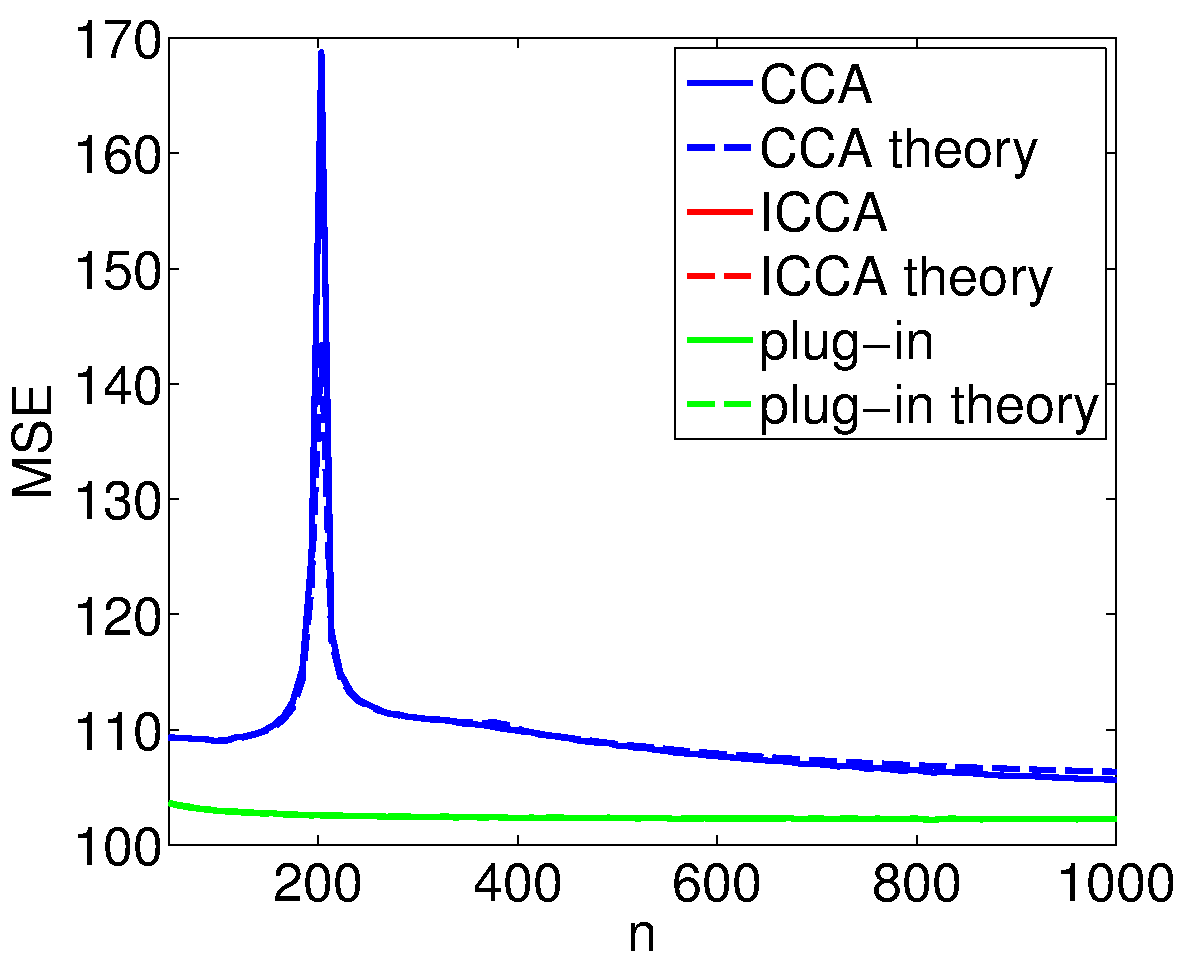
\includegraphics[width=0.45\textwidth]{chpt8_det_reg/figures/regr_mse.pdf}
    \label{fig:chpt8:regr_mse}
  }
  \subfigure[Zoomed-in]{
    \centering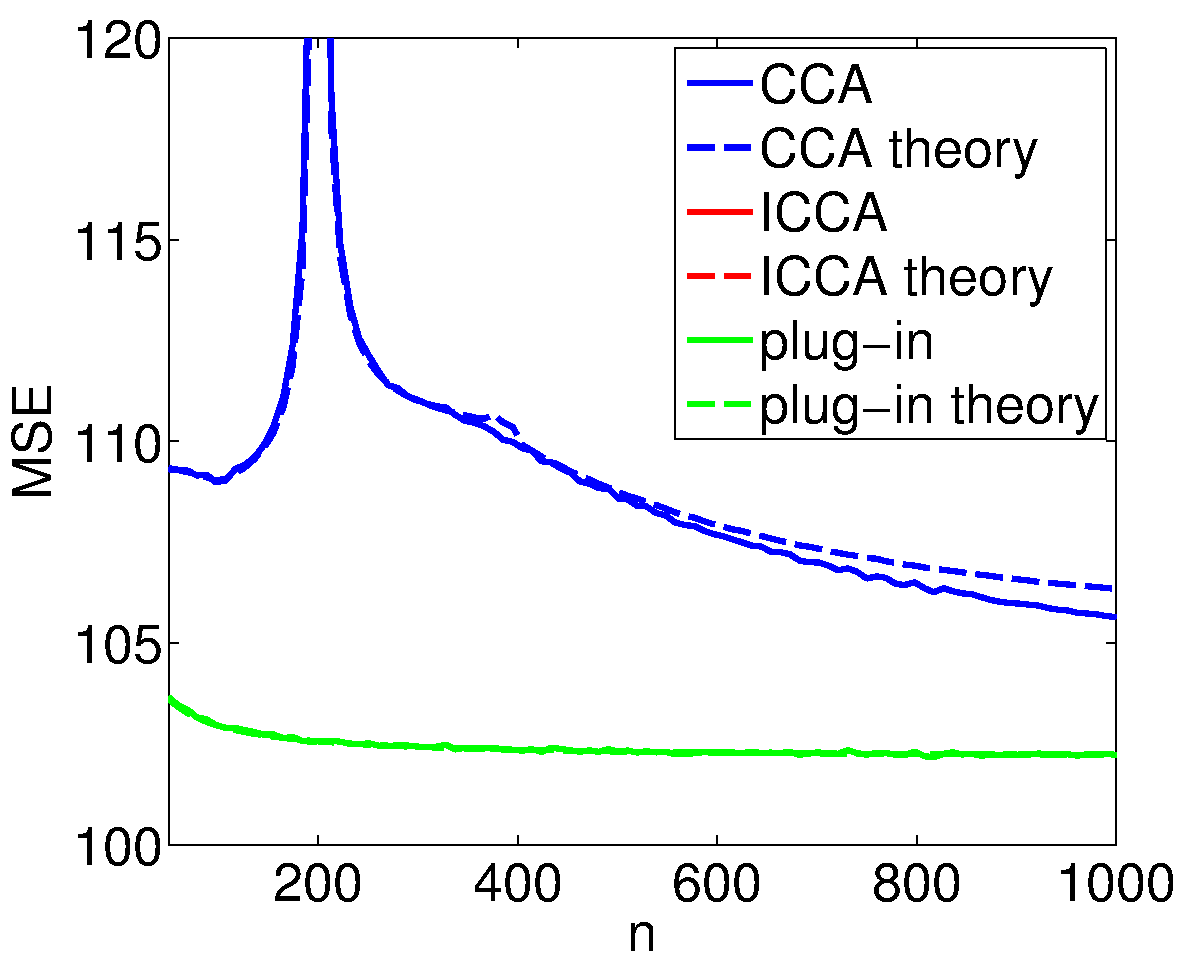
\includegraphics[width=0.45\textwidth]{chpt8_det_reg/figures/regr_mse_zoom.pdf}
    \label{fig:chpt8:regr_mse_zoom}
  }
  \caption{Empirical and theoretically predicted MSE for the plug-in, CCA, and ICCA
    estimators. We use a rank-1 setting where $\kx=\ky=1$, $\tx_1=3$, $\ty_1=4$,
    $p=100$, $q=200$ and $\rho=0.9$. In the rank-1 setting, $\Uktil=\Vktil=1$. The plot on
    the right is a zoomed in version of the plot on the left. The ICCA and plug-in curves
    lie on top of each other, as we showed that the two are equivalent.}
  \label{fig:chpt8:mse}
\end{figure}



\section{LRT Detector Derivation}

Formally, we are given two observation vectors, $x$ and $y$, of different modalities
(having different features). The goal is to design a detector to distinguish between the
$H_1$ hypothesis that the observations contain a target signal and the $H_0$ hypothesis
that the observations are purely noise. 

We consider the Neyman-Pearson setting for detection (see \cite{van1968detection}) where, given a
test observations from (\ref{eq:chpt8:cca_detect_model}), we form $w=[x^H y^H]^H$ by stacking the
individual observations in a column vector. The Neyman-Pearson lemma states that such a
detector takes the form of a LRT
\beq\label{eq:chpt8:lrt}
\Lambda(w) := \frac{f\left(w\,|\,H_1\right)}{f\left(w\,|\,H_0\right)}\detgtrless \gamma,
\eeq
where $\Lambda(w)$ is a test statistic, $\gamma$ is a threshold set to achieve a desired
false alarm rate, and $f$ is the appropriate conditional density of the observation.

The conditional distributions of $w$ under each hypothesis are
\be
\ba
& w|H_0 \sim\mathcal{N}(0,I_d) \\
& w|H_1 \sim\mathcal{N}(0,R_w),\\
\ea
\ee
where $R_w=\E{ww^H}$. Substituting these conditional distributions in (\ref{eq:chpt8:lrt}) , the 
LRT statistic is
\be
\Lambda(w)=\frac{\mathcal{N}(0,R_w)}{\mathcal{N}(0,I_d)},
\ee
which can be simplified to
\beq\label{eq:chpt8:lrt_stat}
\Lambda(w)=w^H\left(I_d-R_w^{-1}\right)w.
\eeq
The covariance matrix of the observation vector is
\be
\ba
&R_w &&=\left[\begin{array}{cc} \Rxx & \Rxy \\ \Rxy^H & \Ryy\end{array} \right] =
\left[\begin{array}{cc} 
\Ux\Tx\Ux^H + I_p &\Ux\Kxy\Uy^H \\\Uy\Kxy^H\Ux^H &\Uy\Ty\Uy^H + I_q
\end{array}\right]\\
&&& = \underbrace{\left[\begin{array}{cc}
\Ux & 0 \\ 0 & \Uy
\end{array}\right]}_{U}
\underbrace{\underbrace{\left[\begin{array}{cc}
\Tx^{1/2} & 0 \\ 0 & \Ty^{1/2}
\end{array}\right]}_{\Theta^{1/2}}
\underbrace{\left[\begin{array}{cc}
    I_{\kx} & \Pxy \\ \Pxy^H & I_{\ky}
\end{array}\right]}_{\widetilde{P}}
\underbrace{\left[\begin{array}{cc}
\Tx^{H/2} & 0 \\ 0 & \Ty^{H/2}
\end{array}\right]}_{\Theta^{H/2}}}_{\widetilde{\Theta}}
\underbrace{\left[\begin{array}{cc}
\Ux^H & 0 \\ 0 & \Uy^H
\end{array}\right]}_{U^H} + I_d\\
&&& = U\Theta^{1/2}\widetilde{P}\Theta^{H/2}U^H + I_d \\
&&& = U\widetilde{\Theta}U^H + I_d. \\
\ea \ee 
Substituting this covariance matrix into the LRT statistic in (\ref{eq:chpt8:lrt_stat})
yields (using the matrix inversion lemma)
\be\ba
&\Lambda_{\text{lrt}}(w) &&=w^H\left(I_d-R_w^{-1}\right)w\\
&&& = w^H\left(I_d-\left(U\widetilde{\Theta}U^H+I_d\right)^{-1}\right)w\\
&&& = w^H\left(I_d-\left(I_d - U\left(\widetilde{\Theta}^{-1}+
    U^HU\right)\right)^{-1}U^H\right)w\\
&&& = w^HU\left(\widetilde{\Theta}^{-1}+I_{k}\right)^{-1}Uw\\
&&& = w^HU\left(\Theta^{-1/2}\widetilde{P}^{-1}\Theta^{-1/2}+I_{k}\right)^{-1}U^Hw\\
&&& = w^HU\Theta^{1/2}\left(\widetilde{P}^{-1}+\Theta\right)^{-1}\Theta^{H/2}U^Hw.\\
\ea\ee
The LRT detector is
\beq\label{eq:chpt8:lrt_detect}
\Lambda_\text{lrt}(w) \detgtrless \gamma_{\text{lrt}}
\eeq
where $\gamma_{\text{lrt}}$ is a threshold set to satisfy 
\be
\Prob{\Lambda_{\text{lrt}}(w) > \gamma_{\text{lrt}}\,|\,H_0} =\alpha,
\ee 
where $\alpha$ is a desired false alarm rate. 

Writing the LRT statistic in this form is desirable for computational reasons. Instead of
inverting $R_w$, which is a $d\times d$ matrix of high dimension, we only need to invert
$k\times k$ matrices.  


\section{CCA Detector Equivalency}
In this section, we will show that the LRT derived above in (\ref{eq:chpt8:lrt_detect})
can be written using the canonical vectors and correlation coefficients found by
CCA.Recall that the matrix of interest in CCA is $\Ccca=\Rxx^{-1/2}\Rxy\Ryy^{-1/2}$ and
that the canonical vectors and correlation coefficients are found by solving the SVD of
$\Ccca=FKG^H$. We begin by manipulating the covariance matrix of $w$.

\be\ba
&R_w &&= \left[\begin{array}{cc}
    \Rxx & \Rxy \\ \Rxy^H & \Ryy
\end{array}\right] = 
\left[\begin{array}{cc}
    \Rxx^{1/2} & 0 \\ 0 & \Ryy^{1/2}
\end{array}\right]\left[\begin{array}{cc}
  I_{p} & \Ccca \\ \Ccca^H & I_{q}
\end{array}\right]\left[\begin{array}{cc}
  \Rxx^{H/2} & 0 \\ 0 & \Ryy^{H/2}
\end{array}\right]\\
&&& = \left[\begin{array}{cc}
    \Rxx^{1/2} & 0 \\ 0 & \Ryy^{1/2}
\end{array}\right]\left[\begin{array}{cc}
    F & 0\\ 0 & G
\end{array}\right]\left[\begin{array}{cc}
  I_{p} & K \\ K^H & I_{q}
\end{array}\right]\left[\begin{array}{cc}
    F^H & 0 \\ 0 & G^H
\end{array}\right]\left[\begin{array}{cc}
   \Rxx^{H/2} & 0 \\ 0 & \Ryy^{H/2}
\end{array}\right].\\
\ea\ee
Using this decomposition, the inverse of the covariance matrix of $w$ is
\be
R_w^{-1} = \left[\begin{array}{cc}
    \Rxx^{-1/2} & 0 \\ 0 & \Ryy^{-1/2}
\end{array}\right]\left[\begin{array}{cc}
    F & 0\\ 0 & G
\end{array}\right]\left[\begin{array}{cc}
    I_{p} & K \\ K^H & I_{q}
\end{array}\right]^{-1}\left[\begin{array}{cc}
    F^H & 0 \\ 0 & G^H
\end{array}\right]\left[\begin{array}{cc}
    \Rxx^{-H/2} & 0 \\ 0 & \Ryy^{-H/2}
\end{array}\right].\\
\ee Recall that the $i$-th canonical vectors returned by CCA are
\be\ba
& \wx^{(i)} = \Rxx^{-1/2}f_i\\
& \wy^{(i)} = \Ryy^{-1/2}g_i\\
\ea\ee
 where $f_i$ and $g_i$ are the left and right singular vectors of $C$ corresponding
to the $i$-th largest singular value, $k_i$, respectively. Define the matrices 
\be\ba
&W_x =\left[\wx^{(1)},\dots, \wx^{(p)}\right]= \Rxx^{-1/2}F\\
&W_y=\left[\wy^{(1)},\dots,\wy^{(q)}\right] = \Ryy^{-1/2}G
\ea\ee
 to be the matrices of canonical vectors
returned by CCA. Using this notation and substituting the expression for $R_y^{-1}$ in the
LRT statistic in (\ref{eq:chpt8:lrt_stat}), we arrive at 
\be\ba
&\Lambda(w)&&= w^H\left(I_d -R_w^{-1}\right)w\\
&&&=w^H\left(I_d - \left[\begin{array}{cc} W_x & 0 \\ 0 & W_y
\end{array}\right]\left[\begin{array}{cc}
    I_{p} & K \\ K^H & I_{q}
\end{array}\right]^{-1}\left[\begin{array}{cc}
  W_x^H & 0 \\ 0 & W_y^H
\end{array}\right]\right)y.\\
\ea\ee 
The above expression is written in terms of the observation $w$, the canonical
vectors $W_x$ and $W_y$ and the correlation coefficients $K$ returned by CCA. This
statistic is exactly equivalent to the LRT statistic derived earlier. Therefore, we
conclude that the CCA basis is the correct basis to use in such low-rank Gauss-Gauss
detection with two datasets.

We can write this detector slightly differently by recalling that the
canonical variates are $\xi_x^{(i)}=\wx^{(i)H}x$ and $\xi_y^{(i)}=\wy^{(i)H}y$. Let
$\xi_x=\left[\xi_x^{(1)},\dots,\xi_x^{(p)}\right]^H$,
$\xi_y=\left[\xi_y^{(1)},\dots,\xi_y^{(q)}\right]^H$, and define
\be 
\xi = \left[\begin{array}{c}\xi_x \\ \xi_y\end{array}\right] =
\left[\begin{array}{cc}W_x^H & 0 \\ 0 & W_y^H\end{array}\right]w. 
\ee
Using this definition and defining
\be
W = \left[\begin{array}{cc}W_x & 0 \\ 0 & W_y\end{array}\right],
\ee
the above detector may be written
\beq\label{eq:chpt8:cca_stat}
\Lambda_{\text{cca}}(\xi) = \xi^H\left(\left(W^HW\right)^{-1}-\left[\begin{array}{cc}
    I_{p} & K \\ K^H & I_{q}
\end{array}\right]^{-1}\right)\xi.
\eeq
In conclusion, we derived a detector that takes the canonical variates as
inputs and uses only the canonical vectors $X$ and the canonical correlation coefficients
$K$ in its test statistic. This detector is
\beq\label{eq:chpt8:cca_detect}
\Lambda_{\text{cca}}(\xi)\detgtrless\gamma_{\text{cca}}
\eeq
where $\Lambda_{\text{cca}}(\xi)$ is defined in (\ref{eq:chpt8:cca_stat}) and
$\gamma_{\text{cca}}$ is a threshold set to satisfy
\be
\Prob{\Lambda_{\text{cca}}(\xi)>\gamma_{\text{cca}}\,|\,H_0}=\alpha,
\ee
where $\alpha$ is the desired false alarm rate. The CCA detector in (\ref{eq:chpt8:cca_detect})
is equivalent to the LRT detector in (\ref{eq:chpt8:lrt_detect}). This is a general proof and is
independent of any data models placed on $w$. That is, in this proof, we did not refer to
the data model in (\ref{eq:chpt8:cca_detect_model}) that motivated the problem.

\subsection{CCA Detector for Data Model (\ref{eq:chpt8:cca_detect_model})}
The above CCA detector was derived for a generic data model. Here we find the canonical
vectors and correlation coefficients for the data model described in
(\ref{eq:chpt8:cca_detect_model}). Under this model, the data covariance matrices are defined in (\ref{eq:chpt8:true_scm})
and their inverses are
\be\ba
&\Rxx^{-1} = \left[\begin{array}{cc}\Ux & \Ux^\perp\end{array}\right]
\left[\begin{array}{cc}\left(\Tx + I_{\kx}\right)^{-1} & 0 \\ 0 &
    I_{p-\kx} \end{array}\right]  \left[\begin{array}{c} \Ux^H \\ \Ux^{H\perp} 
  \end{array}\right] \\
&\Ryy^{-1} = \left[\begin{array}{cc}\Uy & \Uy^\perp\end{array}\right]
\left[\begin{array}{cc}\left(\Ty + I_{\ky}\right)^{-1} & 0 \\ 0 &
    I_{q-\ky} \end{array}\right]  \left[\begin{array}{c} \Uy^H \\ \Uy^{H\perp} 
  \end{array}\right]. \\
\ea\ee 
It follows that the CCA matrix $\Ccca$ is 
\beq\label{eq:chpt8:cca_detec_C}\ba
& \Ccca &&= \Rxx^{-1/2}\Rxy\Ryy^{-1/2}\\
&&& = \Ux\left(\Tx +I_{\kx}\right)^{-1/2}\Tx^{1/2} \Kxy
\Ty^{1/2}\left(\Ty+I_{\ky}\right)^{-1/2}\Uy^H\\
&&& = \Ux\Kxytil\Uy^H.\\
\ea\eeq 
Clearly, when expressed in (\ref{eq:chpt8:cca_detec_C}), $\Ccca$ is a $\min\left(\kx,\ky\right)$ rank
matrix. This implies that there are only $r:=\min\left(\kx,\ky\right)$ non-zero correlation
coefficients. Therefore, there are only $r$ canonical vectors that should be used in a
detector. Define 
\be\ba
&\widetilde{W}_x = W_x(:,1:r)\\
&\widetilde{W}_y = W_y(:,1:r)\\
&\widetilde{K} = K(1:r,1:r)\\
\ea\ee 
as the trimmed canonical vectors and correlation coefficients. Finally define 
\be
\widetilde{W} = \left[\begin{array}{cc}\widetilde{W}_x &0 \\ 0 & \widetilde{W}_y\end{array}\right] 
\ee and
$\widetilde{\xi} = \widetilde{W}^Hw$. Then the CCA detector is 
\beq\label{eq:chpt8:cca_stat_r}
\Lambda_{\text{cca}}(\widetilde{\xi}) =
\widetilde{\xi}^H\left(\left(\widetilde{W}^H\widetilde{W}\right)^{-1}-\left[\begin{array}{cc} I_{r} &
      \widetilde{K} \\ \widetilde{K}^H & I_{r} \end{array}\right]^{-1}\right)\widetilde{\xi},
\eeq
which only uses the $r$ nonzero CCA correlation coefficients and corresponding 
canonical vectors. The matrix inverses here are also much easier to compute as the
matrices are only $2r\times 2r$ instead of $d\times d$. 

\section{Empirical Detectors}

In many applications, the signal matrices $\Ux$, $\Uy$, their SNR matrices $\Tx$, $\Ty$,
and the correlation matrix between datasets $\Pxy$ are unknown and thus the resulting data
covariance matrices are unknown. Therefore, neither the LRT statistic in
(\ref{eq:chpt8:lrt_detect}) or the CCA statistic in (\ref{eq:chpt8:cca_stat_r}), which
relies on $\Ccca$ in (\ref{eq:chpt8:cca_detec_C}), can be computed. In such settings, we
are given training data to estimate any unknown parameters. This section will describe how
to estimate these unknown parameters and use these estimates in the previously derived
detectors. We then will describe how to use ICCA for detection and show its equivalence to
the plug-in LRT detector. Finally, we close with numerical simulations demonstrating that
the ICCA detector achieves the same performance as the plug-in LRT and that the empirical
CCA detector is extremely suboptimal.


\subsection{Plug-in Detector}

To form a realizable LRT detector, we plug-in the parameter estimates in
(\ref{eq:chpt8:param_estims}) into the statistic in
(\ref{eq:chpt8:lrt_stat}). This results in the plug-in LRT statistic
\beq\label{eq:chpt8:plugin_lrt_stat}
\Lambda_\text{plugin}(w)=w^H\widehat{U}\widehat{\Theta}^{1/2}\left(\widehat{\widetilde{P}}^{-1}+\widehat{\Theta}\right)^{-1}\widehat{\Theta}^{H/2}\widehat{U}w.
\eeq

\subsection{Empirical CCA Detector}
Similarly, we create a realizable CCA detector by performing empirical CCA as described in
Section \ref{sec:reg:cca} by forming 
\be
\Cccahat =\Rxxhat^{-1/2}\Rxyhat\Ryyhat^{-1/2}=Q_xI_{p\times n}V_x^HV_y I_{n\times
 q} Q_y^H.
\ee
We then use the largest $r$ singular values and corresponding left and right
singular vectors of $\Cccahat$ to form estimates of the canonical vectors and
correlation coefficients. Specifically, let $\widehat{F}=[\widehat{f}_1,\dots\widehat{f}_r]$ and $\widehat{G}=[\widehat{g}_1,\dots,\widehat{g}_r]$ be the
left and right singular vectors corresponding to the largest $r$ singular values
$\widehat{\kappa}_1,\dots,\widehat{\kappa}_r$. Then the estimates of the canonical vectors
and correlation coefficient 
are
\beq\label{eq:chpt8:emp_cca_detec_params}\ba
& \widehat{\widetilde{K}} = \diag(\widehat{\kappa}_1,\dots,\widehat{\kappa}_r)\\
&\widehat{\widetilde{W}} = \left[\begin{array}{cc}\Rxxhat^{-1/2}\widehat{F} & 0 \\ 0 &
    \Ryyhat^{-1/2}\widehat{G}\end{array}\right]\\
& \widehat{\xi} = \widehat{\widetilde{W}}^Hw.\\
\ea\eeq
We then substitute these estimates into the CCA detector in (\ref{eq:chpt8:cca_stat_r}).
This results in the empirical CCA detector statistic 
\beq\label{eq:chpt8:cca_plugin_stat}
\Lambda_{\text{cca}}(\widehat{\xi}) =
\widehat{\xi}^H\left(\left(\widehat{\widetilde{W}}^H\widehat{\widetilde{W}}\right)^{-1} -
  \left[\begin{array}{cc} I_r & \widehat{\widetilde{K}}\\ \widehat{\widetilde{K}} & I_r \end{array}\right]^{-1}\right)\widehat{\xi}.  
\eeq 

\subsection{ ICCA Detector}

We saw in Chapter 4 that empirical
CCA is suboptimal and that we can avoid much of the performance loss of CCA by
informatively trimming data components before computing the canonical vectors and
correlations. We apply these insights here to form an ICCA detector. We instead form the
matrix 
\be
\Ciccahat = Q_x(:,1:\kx)V_x(:,1:\kx)^HV_y(:,1:\ky)Q_y(:,1:\ky)^H
\ee
and take the top $r$ singular values $\widetilde{\kappa}_1,\dots,\widetilde{\kappa}_r$
and corresponding singular vectors $\widetilde{F}=[\widetilde{f}_1,\dots,\widetilde{f}_r]$ and 
$\widetilde{G}=[\widetilde{g}_1,\dots,\widetilde{g}_r]$. Using this rank-$r$ SVD, we form
informative 
canonical vectors and correlation coefficient similarly as in
(\ref{eq:chpt8:emp_cca_detec_params}). Substituting these informative parameters into the CCA
detector in (\ref{eq:chpt8:cca_stat_r}) results in the ICCA detector statistic  
\beq\label{eq:chpt8:icca_plugin_stat} 
\Lambda_{\text{icca}}(\widetilde{\xi}) =
\widetilde{\xi}^H\left(\left(\widehat{\widetilde{W}}^H\widehat{\widetilde{W}}\right)^{-1} -
  \left[\begin{array}{cc} I_r & \widehat{\widetilde{K}} \\ \widehat{\widetilde{K}} &
      I_r \end{array}\right]^{-1}\right)\widetilde{\xi}.   
\eeq

\subsection{Proof that $\Lambda_{\text{icca}}(\widetilde{\xi})
  \equiv\Lambda_{\text{plug-in}}(w)$}

In this section, we prove that the ICCA detector statistic in (\ref{eq:chpt8:icca_plugin_stat})
is equivalent to the plug-in LRT statistic in (\ref{eq:chpt8:plugin_lrt_stat}). We begin by
manipulating the plug-in detector, relying heavily on the Woodbury matrix inversion
lemma. First we re-write the plug-in detector statistic
\be\ba
&\Lambda_\text{plugin}(w)&&=w^H\widehat{U}\widehat{\Theta}^{1/2}\left(\widehat{\widetilde{P}}^{-1}+\widehat{\Theta}\right)^{-1}\widehat{\Theta}^{H/2}\widehat{U}w\\
&&&=w^H\widehat{U}\left(\widehat{\Theta}^{-1/2}\widehat{\widetilde{P}}^{-1}\widehat{\Theta}^{-1/2}+I_{2r}\right)^{-1}\widehat{U}w\\
&&&=w^H\widehat{U}\left(I_{2r}-\left(\widehat{\Theta}^{1/2}\widehat{\widetilde{P}}\widehat{\Theta}^{1/2}+I_{2r}\right)^{-1}\right)\widehat{U}w.\\
\ea\ee
Next we manipulate the ICCA detector statistic. To do this, we need expressions for the canonical
vectors and correlations in terms of our estimated parameters. First define
\be
\widetilde{C}_\text{icca} = V_x(:,1:\kx)^HV_y(:,1:\ky)
\ee
and its SVD $\widetilde{C}_\text{icca} =
\widehat{U}_{\widetilde{K}}\widehat{\widetilde{K}}\widehat{V}_{\widetilde{K}}$. Note that
these singular values are exactly the singular values of $\Ciccahat$. Therefore, we have
that
\be
\widehat{\widetilde{W}} = \widehat{U}\left(\widehat{\Theta} +
  I_{2k}\right)^{-1/2}\underbrace{\left[\begin{array}{cc} \widehat{U}_{\widetilde{K}} & 0 \\ 0 &
    \widehat{V}_{\widetilde{K}}\end{array}\right]}_{Q_{\widetilde{K}}}.
\ee
Therefore
\be
\widehat{\widetilde{W}}^H\widehat{\widetilde{W}} =
Q_{\widetilde{K}}^H\left(\widehat{\Theta} + I_{2k})\right)^{-1}Q_{\widetilde{K}}
\ee
and
\be
\left(\widehat{\widetilde{W}}^H\widehat{\widetilde{W}}\right)^{-1} =
Q_{\widetilde{K}}^H\left(\widehat{\Theta} + I_{2k})\right)Q_{\widetilde{K}}.
\ee
Also note that
\be
\widetilde{\xi} = \widehat{\widetilde{W}}^Hw.
\ee
Substituting these expressions into (\ref{eq:chpt8:icca_plugin_stat}), we have
\be\ba
&\Lambda_{\text{icca}}(w) &&=
\widetilde{\xi}^H\left(\left(\widehat{\widetilde{W}}^H\widehat{\widetilde{W}}\right)^{-1} -
  \left[\begin{array}{cc} I_r & \widehat{\widetilde{K}} \\ \widehat{\widetilde{K}} &
      I_r \end{array}\right]^{-1}\right)\widetilde{\xi}.   \\
&&&=
w^H\widehat{\widetilde{W}}\left(\left(\widehat{\widetilde{W}}^H\widehat{\widetilde{W}}\right)^{-1}
  - \left[\begin{array}{cc} I_r & \widehat{\widetilde{K}} \\ \widehat{\widetilde{K}} &
      I_r \end{array}\right]^{-1}\right)\widehat{\widetilde{W}}^Hw.   \\
&&& = w^H\widehat{U}\left(\widehat{\Theta}+I_{2r}\right)^{-1/2}Q_{\widetilde{K}}\left(Q_{\widetilde{K}}^H\left(\widehat{\Theta} +
    I_{2r})\right)Q_{\widetilde{K}} -
  \left[\begin{array}{cc} I_r & \widehat{\widetilde{K}} \\ \widehat{\widetilde{K}} &
      I_r \end{array}\right]^{-1}\right)\cdot\\
&&&\,\,\,\,\,\,\,\,Q_{\widetilde{K}}^H\left(\widehat{\Theta}+I_{2r}\right)^{-1/2}\widehat{U}^Hw\\
&&& = w^H\widehat{U}\left(\widehat{\Theta}+I_{2r}\right)^{-1/2}\left(\left(\widehat{\Theta} +
    I_{2r}\right) -  Q_{\widetilde{K}}\left[\begin{array}{cc} I_r & \widehat{\widetilde{K}} \\ \widehat{\widetilde{K}} &
      I_r \end{array}\right]^{-1}Q_{\widetilde{K}}^H\right)\cdot\\
&&&\,\,\,\,\,\,\,\,\left(\widehat{\Theta}+I_{2r}\right)^{-1/2}\widehat{U}^Hw\\
&&& = w^H\widehat{U}\left(I_{2r} -  \left(\widehat{\Theta} +
    I_{2r}\right)^{-1/2}\left[\begin{array}{cc} I_r & \widetilde{C}_\text{icca} \\ \widetilde{C}_\text{icca}^H &
      I_r \end{array}\right]^{-1}\left(\widehat{\Theta} +
    I_{2r}\right)^{-1/2}\right)\widehat{U}^Hw\\
&&& = w^H\widehat{U}\left(I_{2r} -\left(M+I_{2r}\right)^{-1}\right)\widehat{U}^Hw\\ 
\ea\ee
where
\be
M=\left[\begin{array}{cc} \Txhat & \left(\Txhat +
    I_{2r}\right)^{-1/2}\widetilde{C}_\text{icca}\left(\Tyhat +
    I_{2r}\right)^{1/2} \\ \left(\Tyhat +
  I_{2r}\right)^{-1/2}\widetilde{C}_\text{icca}^H\left(\Txhat + 
    I_{2r}\right)^{1/2} &
  \Tyhat \end{array}\right].
\ee
Therefore, we must show that
$M=\widehat{\Theta}^{1/2}\widehat{\widetilde{P}}\widehat{\Theta}^{1/2}$. The block
diagonal entries of $\widehat{\Theta}^{1/2}\widehat{\widetilde{P}}\widehat{\Theta}^{1/2}$
are exactly $\Txhat$ and $\Tyhat$. Therefore, to complete the proof, we must show that
\be
\Txhat^{1/2}\widehat{P}_{xy}\Tyhat^{1/2} = \left(\Txhat +
  I_{2r}\right)^{1/2}\widetilde{C}_\text{icca}\left(\Tyhat + 
    I_{2r}\right)^{1/2}
\ee
Substituting the definition of $\widehat{P}_{xy}$, we have
\be\ba
&\Txhat^{1/2}\widehat{P}_{xy}\Tyhat^{1/2} && = \Txhat^{1/2}\left(\Txhat^{-1/2}\left(\Txhat+I_{\kx}\right)^{1/2}V_x^HV_y\left(\Tyhat +
  I_{\ky}\right)^{1/2}\Tyhat^{-1/2}\right)\Tyhat^{1/2}\\
&&& = \left(\Txhat+I_{\kx}\right)^{1/2}V_x^HV_y\left(\Tyhat +
  I_{\ky}\right)^{1/2}\\
&&& = \left(\Txhat+I_{\kx}\right)^{1/2}\widetilde{C}_{\text{icca}}\left(\Tyhat +
  I_{\ky}\right)^{1/2},\\
\ea\ee
which completes the proof.


\subsection{Rank 1 Numerical Simulations}

We now use numerical simulations to explore the performance of the plug-in LRT detector in
(\ref{eq:chpt8:plugin_lrt_stat}), the empirical CCA detector in (\ref{eq:chpt8:cca_plugin_stat}), and
the ICCA detector in (\ref{eq:chpt8:icca_plugin_stat}) in the rank-1 setting where
$\kx=\ky=1$. Specifically, we wish to empirically verify that the plug-in LRT detector is
equivalent to the ICCA detector. We also wish to explore how the performance of the
CCA detector in compares to that of the plug-in LRT detector. 

To compare the performance of these detectors, we compute empirical ROC curves. To
compute an empirical ROC curve, we first generate  two random signal vectors, $\Ux=u_x$ and
$\Uy=u_y$, by taking the first left singular vector of two appropriately sized random
matrices with i.i.d. $\mathcal{N}(0,1)$ entries. In this simulation we make the
simplifying assumption that $\tx_1=\ty_1=\theta$. Given a desired SNR, correlation $\rho=\Pxy$,
and random $u_x$ and $u_y$, we generate $n$ training samples of $\xii$ and $\yii$ from the
$H_1$ hypothesis in (\ref{eq:chpt8:cca_detect_model}). Using these training samples, we form
estimates $\widehat{U}$, $\widehat{\Theta}$, $\widehat{\rho}$, $\Rxxhat$, $\Ryyhat$, and
$\Rxyhat$ as described in Section \ref{sec:param_estims}.

We then generate a desired number of test samples from each hypothesis using
(\ref{eq:chpt8:cca_detect_model}). For each test sample, we compute the test statistic for the
plug-in LRT, empirical CCA, and ICCA detectors in (\ref{eq:chpt8:plugin_lrt_stat}),
(\ref{eq:chpt8:cca_plugin_stat}), and (\ref{eq:chpt8:icca_plugin_stat}), respectively. Using Fawcett's
\cite{fawcett2006introduction} `Algorithm 2', we compute an empirical ROC curve by first
sorting the test statistics for a given detector. At each statistic, we log a ($P_F$,
$P_D$) pair by counting the number of lower scores generated from each hypothesis. This is
repeated for multiple realizations of $u_x$ and $u_y$, generating multiple empirical ROC
curves for each detector. We refer to a single empirical ROC curve corresponding to a
realization of $u_x$ and $u_y$ as a trial. We then average the empirical ROC curves for a
detector over multiple trials using Fawcett's \cite{fawcett2006introduction} `Algorithm
4'. This performs threshold averaging by first uniformly sampling the sorted list of all
test scores of ROC curves and then computing ($P_F$, $P_D$) pairs in the same way as
`Algorithm 2'.

To compare the ROC curves of different detectors, we use the area under the ROC curve
(AUC) statistic. The AUC statistic ranges between 0.5, which represents a random guessing
detector, and 1.0, which represents a detector that can perfectly distinguish between the
two hypotheses. We compute the ROC curves and their respective AUC for many values of the
number of training samples, $n$, and SNR $\theta=\tx_1=\ty_1$. We present the AUC
results in the form of a heatmap for two different values of $\rho$ for each of the
detectors. Figure \ref{fig:chpt8:auc_high_rho} presents results for $\rho=0.8$ and Figure
\ref{fig:chpt8:auc_low_rho} presents results for $\rho = 0.2$.

\begin{figure} 
  \subfigure[Plug-in LRT]{
    \centering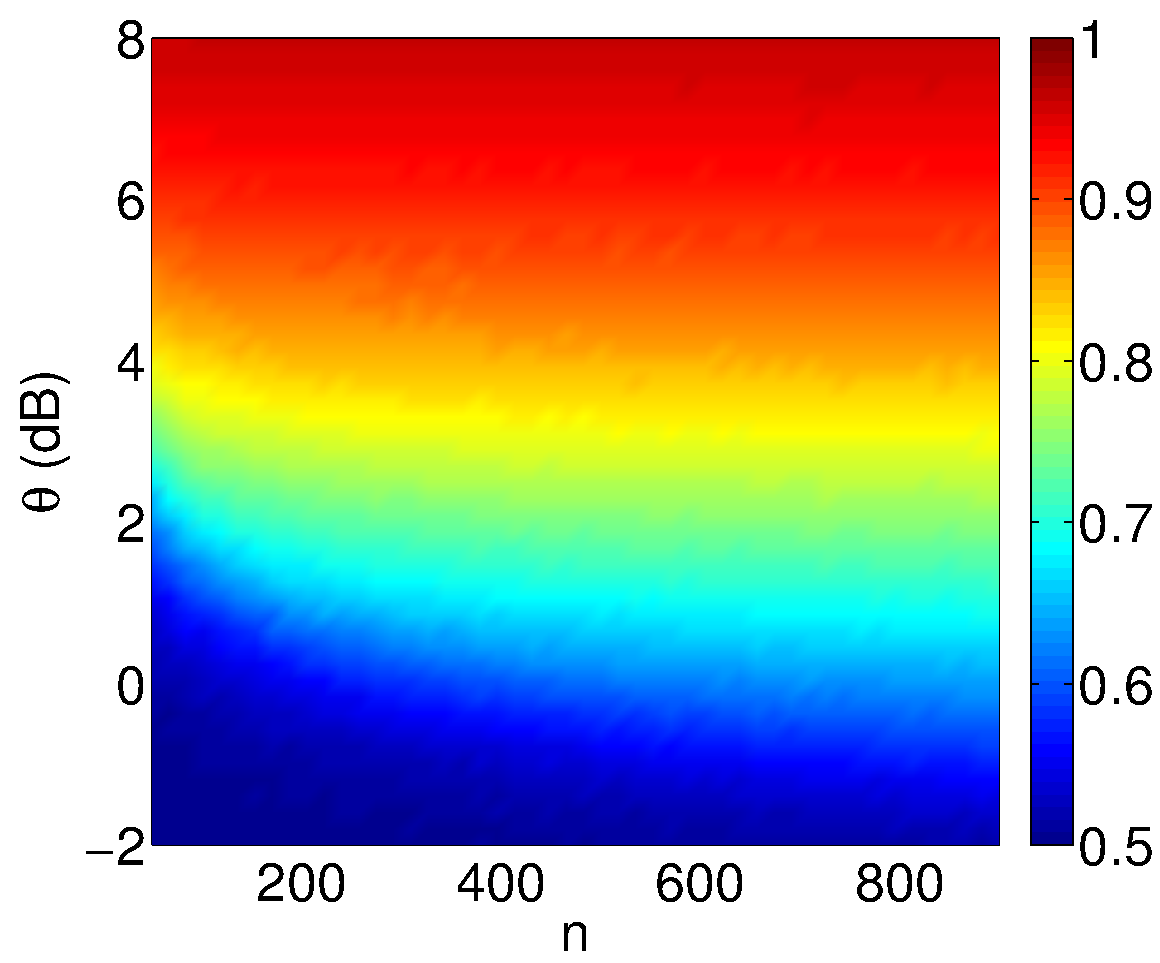
\includegraphics[width=0.45\textwidth]{chpt8_det_reg/figures/auc_lrt_high_rho.pdf}
    \label{fig:chpt8:auc_lrt_high_rho}
  }
  \subfigure[ICCA]{
    \centering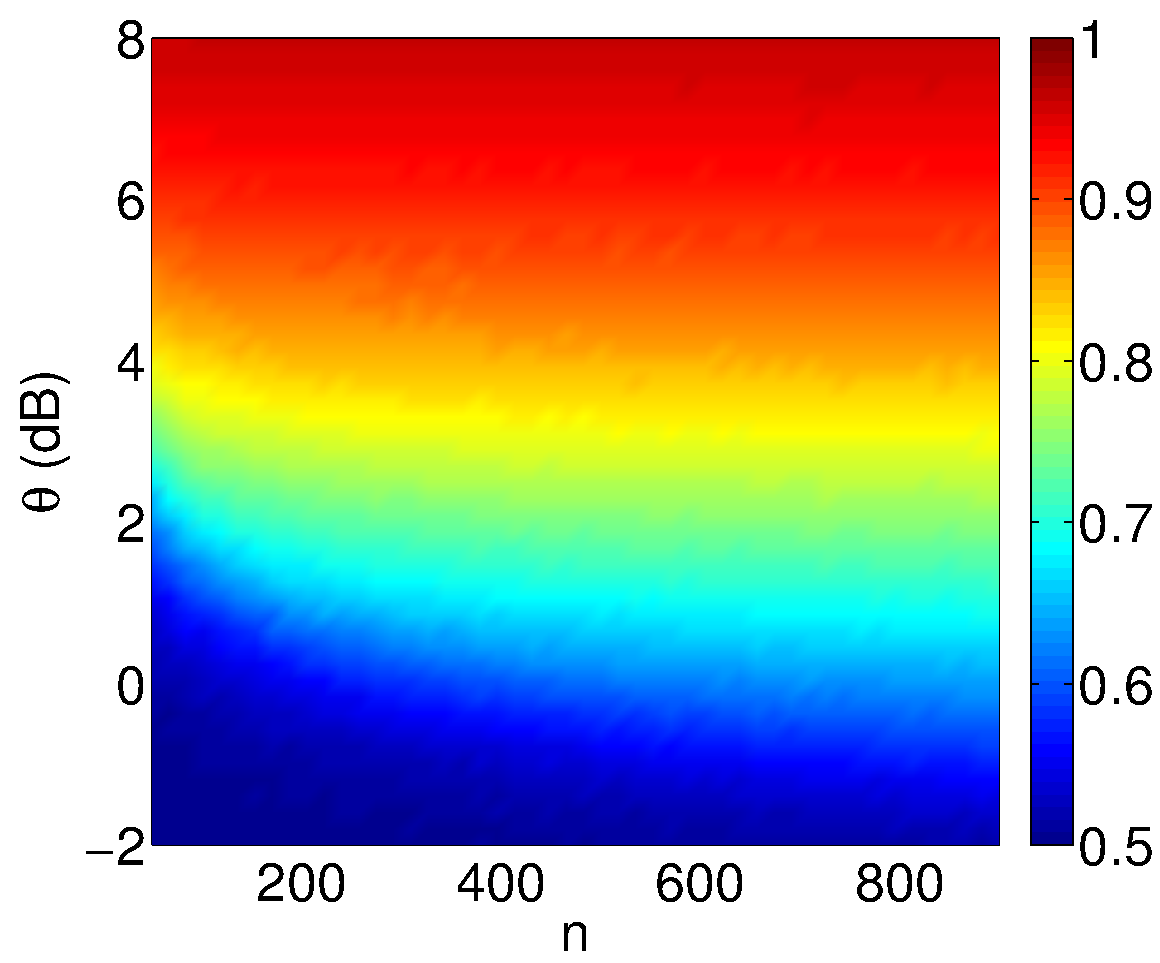
\includegraphics[width=0.45\textwidth]{chpt8_det_reg/figures/auc_icca_high_rho.pdf}
    \label{fig:chpt8:auc_icca_high_rho}
  }
  \subfigure[Empirical CCA]{
    \centering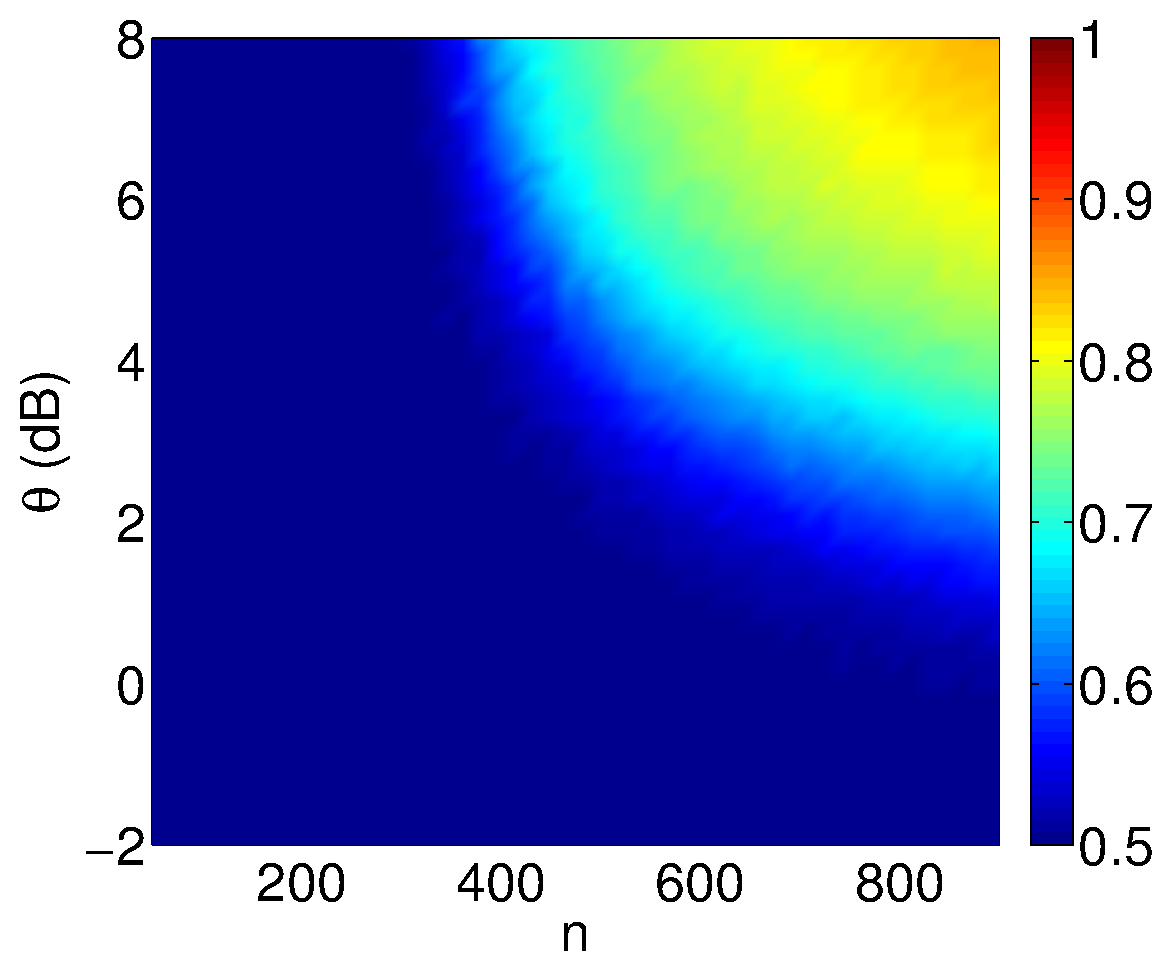
\includegraphics[width=0.45\textwidth]{chpt8_det_reg/figures/auc_cca_high_rho.pdf}
    \label{fig:chpt8:auc_cca_high_rho}
  }
  \caption{AUC results for the plug-in LRT, empirical CCA, and ICCA detectors in
    (\ref{eq:chpt8:plugin_lrt_stat}), (\ref{eq:chpt8:cca_plugin_stat}), and
    (\ref{eq:chpt8:icca_plugin_stat}), respectively. Empirical ROC curves were simulated using
    $2000$ test samples for each hypothesis and averaged over $50$ trials using
    algorithms 2 and 4 of \cite{fawcett2006introduction}. Simulations parameters were
    $p=200$, $q=150$, and $\rho=0.8$. Each figure plots the AUC for the average ROC curve
    at a different values of SNR, $\theta=\tx_1=\ty_1$, and training samples, $n$.}
  \label{fig:chpt8:auc_high_rho}
\end{figure}

\begin{figure} 
  \subfigure[Plug-in LRT]{
    \centering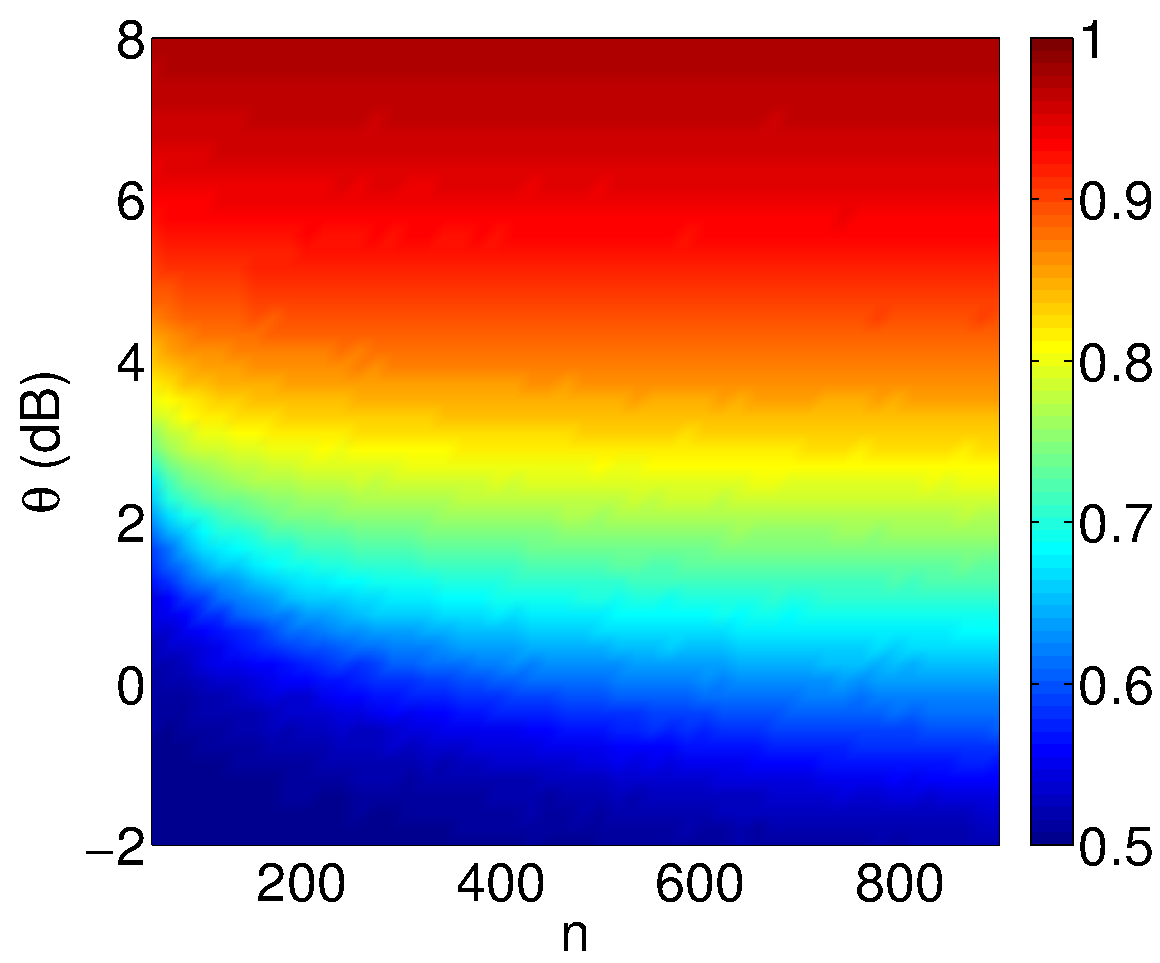
\includegraphics[width=0.45\textwidth]{chpt8_det_reg/figures/auc_lrt_low_rho.pdf}
    \label{fig:chpt8:auc_lrt_low_rho}
  }
  \subfigure[ICCA]{
    \centering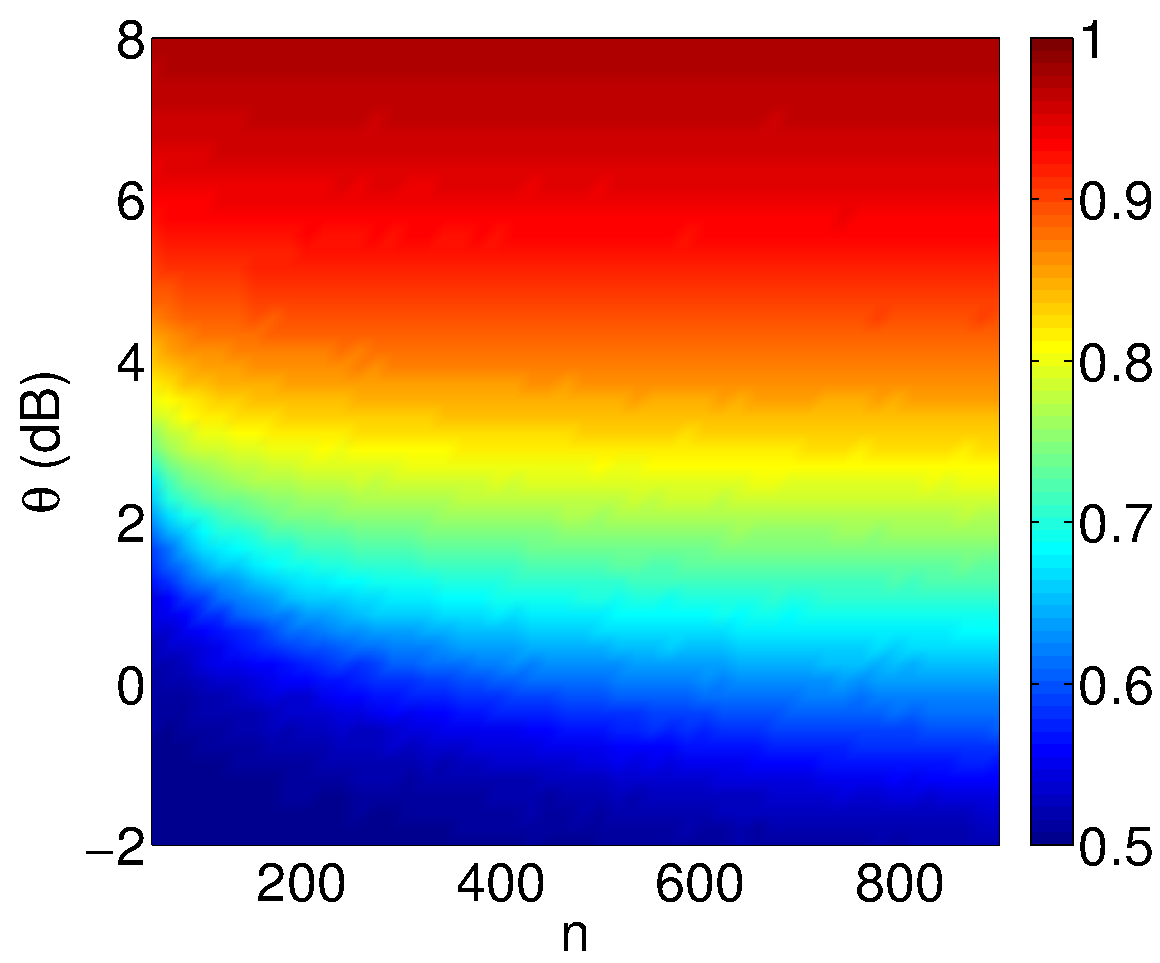
\includegraphics[width=0.45\textwidth]{chpt8_det_reg/figures/auc_icca_low_rho.pdf}
    \label{fig:chpt8:auc_icca_low_rho}
  }
  \subfigure[CCA]{
    \centering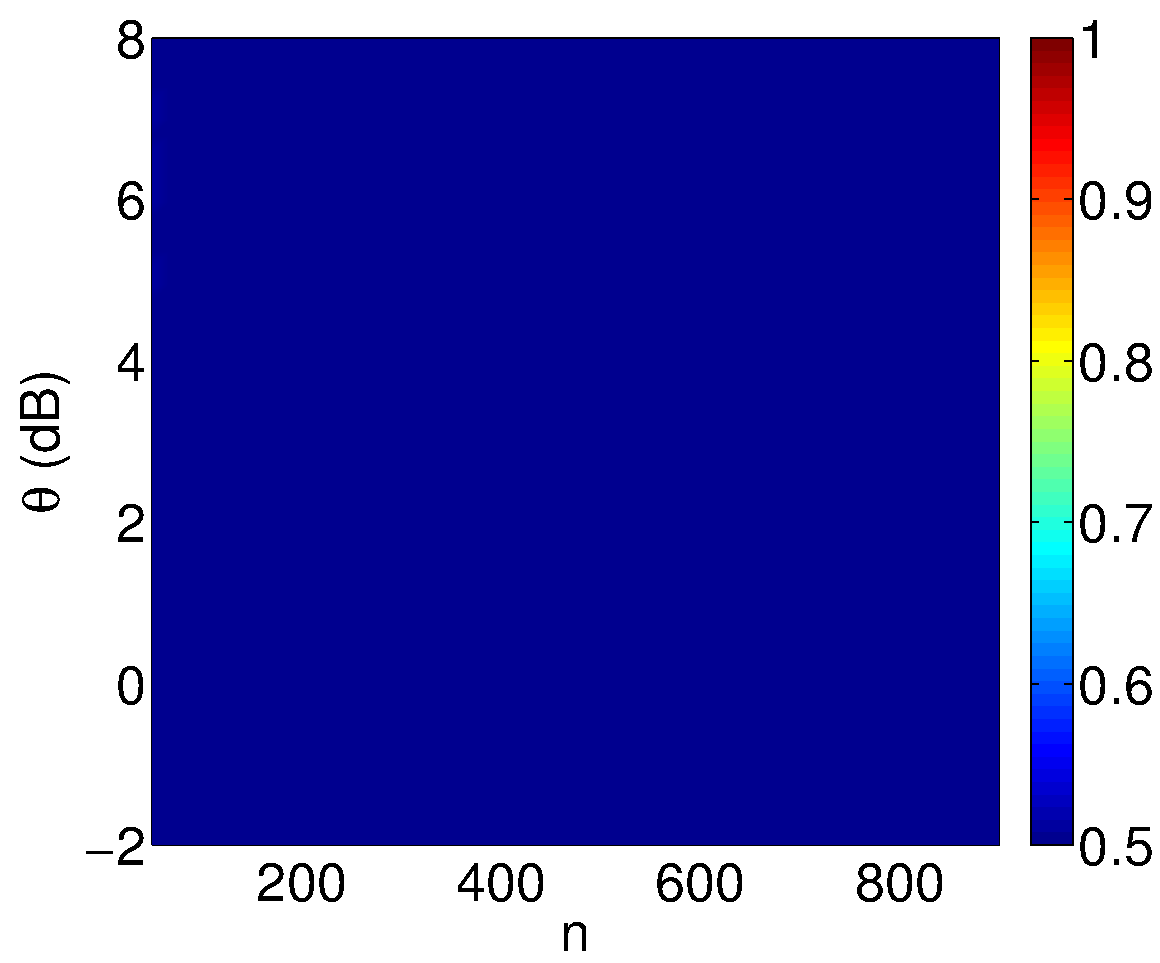
\includegraphics[width=0.45\textwidth]{chpt8_det_reg/figures/auc_cca_low_rho.pdf}
    \label{fig:chpt8:auc_cca_low_rho}
  }
  \caption{AUC results for the plug-in LRT, empirical CCA, and ICCA detectors in
    (\ref{eq:chpt8:plugin_lrt_stat}), (\ref{eq:chpt8:cca_plugin_stat}), and
    (\ref{eq:chpt8:icca_plugin_stat}), respectively. Empirical ROC curves were simulated using
    $2000$ test samples for each hypothesis and averaged over $50$ trials using
    algorithms 2 and 4 of \cite{fawcett2006introduction}. Simulations parameters were
    $p=200$, $q=150$, and $\rho=0.2$. Each figure plots the AUC for the average ROC curve
    at a different value of SNR, $\theta=\tx_1=\ty_1$, and training samples, $n$.}
  \label{fig:chpt8:auc_low_rho}
\end{figure}

\begin{figure} 
  \centering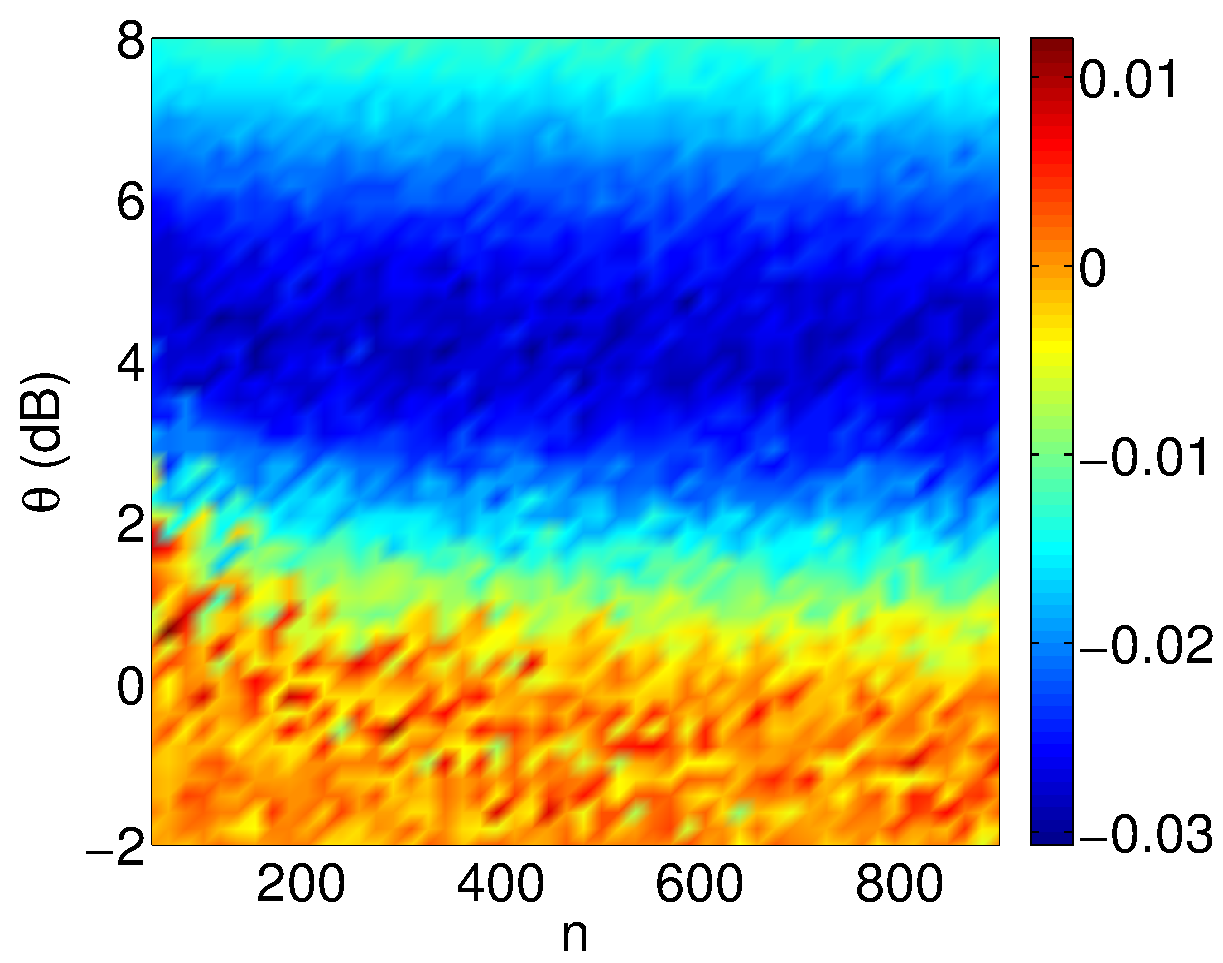
\includegraphics[width=0.45\textwidth]{chpt8_det_reg/figures/auc_icca_diff.pdf}
  \label{fig:chpt8:auc_cca_diff}
  \caption{Difference between ICCA AUC heatmaps in Figures \ref{fig:chpt8:auc_cca_low_rho}
  and \ref{fig:chpt8:auc_cca_high_rho}. Positive values indicate when the setting of
  $\rho=0.8$ achieves a higher AUC. Negative values indicate when the setting of
  $\rho=0.2$ achieves a higher AUC.}
  \label{fig:chpt8:auc_diff}
\end{figure}


Evident in both Figures \ref{fig:chpt8:auc_high_rho} and \ref{fig:chpt8:auc_low_rho}, the ICCA
detector exhibits the same AUC performance as the plug-in LRT for both values of
$\rho$. This confirms the derivation in the above section. In Figure
\ref{fig:chpt8:auc_high_rho}, we observe that the CCA detector is extremely suboptimal in the
sample and SNR regime presented. When $n<350=p+q$, the CCA detector degrades to random
guessing, evident in an AUC of 0.5. The results presented in Chapter
4 show that in this sample poor regime, the correlation coefficient
estimate returned by CCA is deterministically 1. It is of no surprise that the subsequent
CCA detector is useless in this regime. Even when $n>p+q$, the CCA detector achieves a
lower AUC than the ICCA detector. The ICCA detector can tolerate a much lower SNR to achieve
the same AUC performance as the CCA detector.

When decreasing $\rho$ in Figure \ref{fig:chpt8:auc_low_rho}, the CCA detector observes an even
further performance loss. In the training sample and SNR parameter regime presented,
the CCA detector achieves an AUC of 0.5, indicating it is useless in detection. We plot
the difference between the ICCA AUC heatmaps for the two choices of $\rho$ in Figure
\ref{fig:chpt8:auc_diff}. For small values of $\theta$, the larger value of $\rho$ results in
the better performance while for large values of $\theta$, the smaller value of $\rho$ results
in better performance. Decreasing $\rho$ makes the observations $x$ and $y$ more
independent, thereby containing more information and increasing detection
performance. Therefore, this observation is intuitive. When the SNR is large, we have more
reliable information for larger $\rho$. When the SNR is small, the correlation between the
datasets helps to better detect the signal. We can think of this as SNR boosting.

These results are particularly surprising because we began this chapter by deriving the
fact that the LRT detector is equivalent to the CCA detector. However, when using
parameter estimates, the empirical CCA detector no longer is equivalent to the plug-in
detector. As many applications require estimating the covariance matrices used in CCA,
this is an extremely undesirable property of CCA. However, using only the informative
components from our training data, as ICCA does, results in equivalent performance as the
plug-in LRT detector. This performance loss of the empirical CCA detector can be avoided
by instead using ICCA.

